%%
%% This is file `mcmthesis-demo.tex',
%% generated with the docstrip utility.
%%
%% The original source files were:
%%
%% mcmthesis.dtx  (with options: `demo')
%% !Mode:: "TeX:UTF-8"
%% -----------------------------------
%%
%% This is a generated file.
%%
%% Copyright (C)
%%     2010 -- 2015 by latexstudio
%%     2014 -- 2016 by Liam Huang
%%     2014 -- 2016 by latexstudio.net
%%
%% This work may be distributed and/or modified under the
%% conditions of the LaTeX Project Public License, either version 1.3
%% of this license or (at your option) any later version.
%% The latest version of this license is in
%%   http://www.latex-project.org/lppl.txt
%% and version 1.3 or later is part of all distributions of LaTeX
%% version 2005/12/01 or later.
%%
%% This work has the LPPL maintenance status `maintained'.
%%
%% The Current Maintainer of this work is Liam Huang.
%%

\documentclass{mcmthesis}
\mcmsetup{CTeX = true,   % 使用 CTeX 套装时,设置为 true
        tcn = 123456789, problem = C,% 队伍控制号码,接受一个字符串作为值;选题,接受一个字符串作为值;
        sheet = true, %为真时将输出摘要页,否则不输出;默认为 true。
        color = black,  %设置控制页的题目号的颜色
        titleinsheet = true, %为真时将在摘要页输出标题,否则不输出;默认为 false。
        keywordsinsheet = true,%为真时将在摘要页输出关键字,否则不输出;默认为 false。
        titlepage = true,%为真时将输_{}出标题页,否则不输出;默认为 true。
        abstract = true}%为真时将在标题页输出摘要和关键词,否则不输出;默认值为 true。
 
\usepackage{palatino}  %控制正文字体,若是不喜欢可以注释掉。
%\usepackage{lipsum}  %生成随机文本
%%%%%%绘图包%%%%%%
\usepackage{tikz}
\usepackage{subfigure} %%并排图片
\usepackage{graphicx}  
%\usepackage{subcaption}
\usepackage{caption}
%%%%%制表宏包%%%%%%%
\usepackage{diagbox} 
\usepackage{multirow} 
\usepackage{multicol} 
\usepackage{arydshln}
\usepackage{booktabs}  %%三线表
\usepackage{multirow}
\usepackage{floatrow}  %%并排表格
%%%%添加表格脚注%%%%%
\usepackage{footnote}
%%%%%修改行距、缩进%%%%%
\usepackage{indentfirst}
\usepackage{changepage}
\usepackage[english]{babel}
 \usepackage{setspace} %%间距
 \usepackage{array} %%行距
%%%%%加粗字体%%%%%%%
\usepackage{bm}
%%%%%数学字体%%%%%%%
\usepackage{mathptmx}
\usepackage{txfonts}
%%%%%%经纬度%%%%%%%%
\usepackage{siunitx} 
%%%%%%矩阵%%%%%%%
\usepackage{amsmath} 



%%%%%%%标题页%%%%%%%
\title{The Paper Title}
%\author{}
%\date{\today}

\makeatletter
\renewcommand*\l@section{\@dottedtocline{1}{12pt}{12pt}}
\makeatother

\begin{document}
%%%%%%%摘要内容%%%%%%%
\begin{abstract}
%%%%%关键字%%%%%%
\begin{keywords}
keyword1; keyword2
\end{keywords}
\end{abstract}
\maketitle
%\tableofcontents 
%生成目录
\tableofcontents
\newpage  %%换页


%%%%%%%正文%%%%%%%%
\section{Introduction}
\subsection{Problem Background} %%问题背景
%%众所周知,阿片类药物是一把双刃剑。它既能够帮助患者减轻病痛,也能够使人上瘾。原因是阿片类药物可以为他们带来短暂的快乐,但由于每个人对药物的耐受性不同,药物摄入量越大,这种令人愉快的感觉就越强,这也是导致阿片类药物被滥用的根本原因。当今,美国正经历一场因滥用阿片类药物而带来的危机,我们将面临前所未有的挑战。
As we know, the Opioid is a double-edged sword.It can help patients reduce their pain and also makes people addicted to the Opioid.The reason is that Opioids can bring them short pleasure.However,becuase each people has different tolerance to drugs,when the intake of the drug gets more and more,people will have a stronger sense of plesure.This is the root cause of the abuse of opioids.Today, the United States is experiencing a crisis caused by the abuse of opioids.We will always face unprecedented challenges.There are some of the consequences of the abuse of opioids.
\begin{itemize}
	\item \textbf{Neonatal Abstinence Syndrome} \\%%新生儿戒断综合征
	Neonatal Abstinence Syndrome usually appears 48 to 72 hours after the birth of an infant.The reason is that pregnant women take too much opioids during pregnancy to reduce their pain. \\
	 %%新生儿戒断综合征通常在婴幼儿出生后 48~72 小时出现,病因是孕妇在怀孕期间服用过量的阿片类药物来缓解疼痛。
	\item \textbf{Abuse of opioid lead to an increase in crime rates.} \\
	The opioid is consist of natural, synthesis and semi-synthetic.Synthetic opioid include Fentanyl and Methadone.Otherwise, Semi-synthetic Opioid include Heroin.The former is easier to transport than the latter.Therefore, this is more likely to lead to an increase in crime rate. \\
	%%阿片类药物可以分为天然类、合成类和半合成类,其中合成类包括芬太尼;半合成类包括海洛因,前者比后者要方便运输,因此犯罪率要更高。
	\item \textbf{A huge impact on the demographic structure of the United States.} \\ %%对美国人口结构产生巨大冲击
	In the US, there is a tendency to abuse opioids for people of all ages.And it will increase the mortality rate of the American people.
	%%药物已经成为美国面临的国家危机之一,美国各个年龄层的人口在都有过量摄入阿片类药物的趋势,这会增加国民的死亡率和成瘾性
\end{itemize}
%%%%%插背景图%%%%%%%
\begin{figure}[!h]
	\small
	\centering
	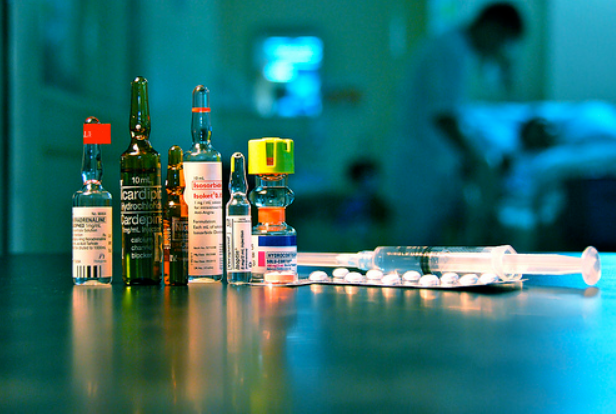
\includegraphics[width=10cm]{back}
	\caption{Drugs} \label{fig:aa}
\end{figure}
\newpage %%换页

%%%%%%%问题分析%%%%%%%
\section{Problem Analysis} 

\subsection{Commonly Abused Drugs Charts }%%常见被滥用的药物分类

%%%常见被滥用的阿片类药物图表%%%%%
\begin{table}[htbp]
	\centering
	\caption{ Commonly Abused Opioid Drugs Charts}
	\begin{tabular}{p{3cm}p{7cm}p{3cm}} %%设置宽度
		\addlinespace
		\toprule
		Drug & Description & Type \\%%药物名&&描述&&分类
		\midrule
		  \textit{Morphine}  & an opioid analgesic drug &  Natural   \\%%吗啡
		  \textit{Codeine}  & an alkaloid present in opium &    Natural      \\      %%可待因
		  \textit{Heroin}   & a potent analgesic drug &  Semi-Synthetic  \\          %%海洛因
		  \textit{Hydrocodone}  & a semi-synthetic opioid drug &  Semi-Synthetic  \\          %%氢可酮
		  \textit{Fentanyl}  & a potent analgesic drug &  Synthetic  \\          %%芬太尼
		  \textit{Methadone}  & an opioid drug & Synthetic   \\          %%美沙酮
		  \textit{Pethidine}  & an artificial anesthetic drug & Synthetic   \\          %%哌替啶
		  \textit{Endorphin}  & an endogenous opioid drug & Endogenous  \\         %%脑内啡
		  \textit{Dynorphins}  & an endogenous opioid drug & Endogenous   \\        %%强啡肽
		\bottomrule
	\end{tabular}%
	\label{tab:addlabel}%
\end{table}%


%%%%%%%问题重述%%%%%%
\subsection{Restatement of The Problem}
\begin{itemize}
	\item[-] \textbf{Needing to solve the first question.} \\ %%解决第一问的思路
	\begin{itemize} %%%二级编号
	\item[-] According the original datasets,We need to build a mathematical model to describe the relationship between every year and the county which using opioids.\\
	%%根据原始数据集,我们需要建立一个数学模型来描述每年和使用阿片类药物的县之间的关系。
	\item[-]  According the  mathematical model,We can get the earliest location reported to be using opioid in five states.  \\
	%%根据这个模型,我们就能够得到五个州中的哪几个县最早使用阿片类药物的具体位置。
	\item[-]  	If you continue to follow the increase in the year.Abuse of opioids will must bring irreversible harm to American society.It will become the United States government’s concerns about this questions. \\
	%%如果按照年份增加的情况继续下去,滥用阿片类药物势必会为美国社会带来不可逆转的伤害,它们将成为美国政府对这一问题的担忧。
	\item[-] We use the mathematical model to predict what will happen in the future.
	%%使用这个模型预测未来发生的情况
	\end{itemize}
\newpage

	\item \textbf{Needing to solve the second question.} \\ %%解决第二问的思路
	\begin{itemize} %%%二级编号
      \item[-] Need to explain the situation in which the opioids are abused up until now.\\  %%解释造成至今滥用阿片类药物的情况
      \item [-] Need to find out what causes the social crisis result in by the abuse of opioid.\\%%需要找出是哪些因素导致阿片类药物被滥用而引发的社会危机。
    \end{itemize}
		
	\item \textbf{Needing to solve the third question.} \\ %%解决第三问的思路
	   \begin{itemize}
	   	\item[-] Optimize the model created by the first question and the second question.%%优化之前提到的模型
	   \end{itemize}
\end{itemize}


%%%%%%我们的思路%%%%%%%%%
\subsection{Overview of Our Work} %%可以设计一个解决所有问题的框架图,然后全部删掉下面的所有子序号
\begin{itemize}
\item \textbf{The idea of solving the first problem.} \\ %%解决第一问的思路
First of all, We need to use the eight years from 2010 to 2017 as the time variable and the total number of drug reports county as independent variables. And then we perform data preprocessing on the total number of drug reports county.Selecting the counties that rank the  top 4 position in five states.At the same time, We will mark these counties on the map.According to these pictures,We can observe the earliest location reported to be using opioid in five states from these eight pictures.\\

%%首先,我们团队解决问题时的思路是,确定五个州中被调查机构报道最早使用阿片类药物的地理位置。因此,我们需要根据原始数据集求出具体的经纬度。在删除异常数据之后,我们接着将 2010~2017 这八年作为时间变量,将每个州下辖的每个县的所有药物被报道使用的次数作为自变量。其次,我们对每个县的所有药物被报道使用的次数进行数据预处理,筛选出每个州排名靠前的4个县(暂定),将其在地图上标出。根据年份,一共可以得出八张图。我们可以通过这八张图直观地看出五个州中的哪几个县最早使用阿片类药物的具体位置。


\item  \textbf{The idea of solving the second problem.}\\%%解决第二问的思路

\item  \textbf{The idea of solving the third problem.} \\%%解决第三问的思路
\end{itemize}

%%%%%问题假设%%%%%
\section{Assumptions and Notations}
\subsection{Assumptions}

\begin{itemize}
	\item \textbf {Assuming all the latitude and longitude in the US is valid,} but not in the US are invalid data. %%假设在美国之内的经纬度是有效的,不在则无效
	\item \textbf{Assuming the earliest use of opioids in five states}is gradually spreanding to the other contry. %%假设最早出现的位置会向其他地方扩散
	\item  \textbf{Assuming each states only related with the county it administers.} %%假设每一个州只与它下辖的县有联系,独立性
	%\item  \textbf{?????}  \\
\end{itemize}

%%%%%符号定义%%%%%
\subsection{Notations}
\textbf {Here is we need to use the symbols description in this paper.} \\ 

\begin{tabular}{cp{0.8\textwidth}}	
	\toprule
	Symbols & Description \\
	\midrule
	$n$ & each small area of a polygon \\      %%组成多边形的每个小三角形
	$k$ & predicted object\\      %%预测对象
	$p$ & predicted standard\\      %%预测标准
	${G_i}({x_i},{y_i})$ & the geometric center of gravity of a small triangle \\ %%小三角形的几何重心坐标
	${G_j}({x_j},{y_j})$ & the geometric center of gravity of the polygon \\ %%多边形的几何重心坐标
	${\sigma _i}$ & size of each small area\\  %%小三角形的面积
	${\sigma _j}$ & size of each polygon\\  %%多边形的面积
	${\Delta _{ij}}$ & the reference sequence\\ %%预测对象和预测标准组成的参考序列 →  $ x_p $ 出现在 logistc model
	$ {\delta _{ij}} $ & the relationship between predicted object and predicted standard\\%%灰色关联度
	$g(x)$ & a sigmod activation function \\%%激活函数
	$f_m$ &  common factor\\ %%公共因子   
	$ {\varepsilon _p}$ &  special factor\\   %%特殊因子
	$F$ &  common factor vector\\ %%公共因子向量 	
	$\varepsilon$ & pecial factor vector  \\ %%特殊因子向量 
	$ A$ &  load factor matrix\\ %%载荷因子矩阵 g(x)
	\bottomrule
\end{tabular}
%\newpage %%换页


\section{Data Processing}
%%%%%%介绍Geopy地理工具包及数学原理%%%%%%
For the datasets provided by the title,We tried to preprocess the datasets to use the Geopy-Geocoding-Toolkit in the Python.The Geopy-Geocoding-Toolkit
converts geocoding into geographic coordinates -- latitude and longitude.Because Geopy is calling other third-party Map APIs to get geocoded information,then it converts to exact latitude and longitude coordinates.In essence,This is the mathematical principle used to calculate the two-point distance of the Earth's elliptical model. \\

%%%%%%插图%%%%%%%
\begin{figure}[!h] %标题强制上移
	\small
	\centering
	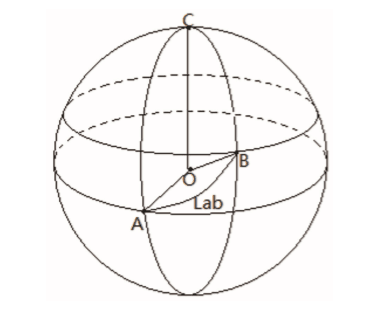
\includegraphics[width=6cm]{Earth}
	\caption{Earth Model} \label{fig:Earth model}
\end{figure}

%%%%%%公式%%%%%%%

\noindent Thus, a simple form of the equation representing the geometric state of the Earth's space.We use the \textbf {WGS-84} ellipsoidal standard.\\


\noindent The Geospatial Geometry for the earth equation is :\\
%%这是地理空间几何方程
\noindent Since, $\bm a$ means the radius of the equator ,  $\bm b$ is the polar axis radius, \\%% a 是赤道半径,b 是极轴坐标
\begin{equation}
\frac{x^2+y^2}{a^2}+\frac{z^2}{b^2} = 1  %地理空间几何方程
\end{equation}
\noindent for some, $\bm a $ = 6378137.000 m, $\bm b$ = 6356752.314 m. \\

\subsection{Data Cleaning} %%数据清洗
%%%%%%正文%%%%%%
After data preprocessing,We observed a small amount of abnormal data appeared in the datasets.These anomalous data have an obvious feature, their geocoded information is not in the United States.This also causes the latitude and longitude after the conversion is not within the United States.
%\newpage
\begin{itemize}
	\item \textbf {Sort the Original Datasets} \\ %%排序
	 Firstly, We use Microsoft Excel to sort the five states and counties of the original datasets.
	
	\item \textbf {Abnormal Value Processing}  \\ %%删除异常数据
	Secondly,We observed a small amount of abnormal data appearing,these anomalous datas have an obvious feature. Its geocoded information is not in the USA, then we will delete thiese datas.
    
    \item \textbf{Get Location Latitude and Longitude} \\%%输出地理位置坐标	
    After deleting the abnormal datas, We use the Geopy-Geocoding-Toolkit in the Python to output latitude and longitude coordinates in the datasets.
  
\end{itemize}


\subsection{Data Visualization}  %%数据可视化
%%此处使用数据可视化的方法将这些经纬度坐标标记在地图上,我们可以很直观地看出

%%%%%%插图(待定)%%%%%%%
\begin{figure}[!h] %标题强制上移
\small
\centering
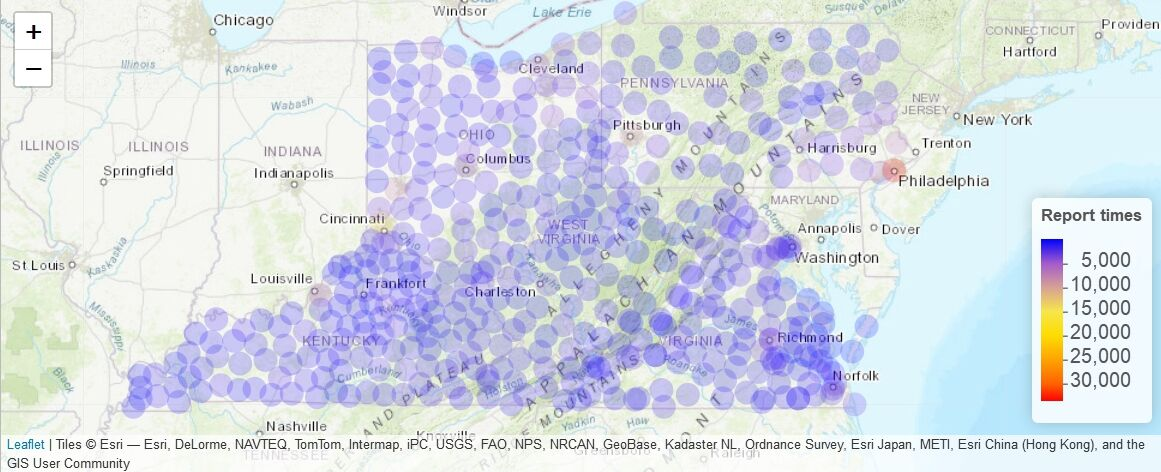
\includegraphics[width=14cm]{Report}
\caption{Using The Geopy-Geocoding-Toolkit deal with Data} \label{fig:Report Times}
\end{figure}









%%%%%%%模型的建立和求解%%%%%%
\section{Model Design}
\subsection{Model 1 - The Mathematical Model of the Relationship between County Location and Opioids} %%县的位置与阿片类药物之间的关系
\begin{itemize}
 \item \textbf{The Polygonal Geometric Center of Gravity Model} \\%%多边形几何模型
  Our team think that choose the counties that rank the top 4 about using opioids.So, we can infer the location of the counties where the opioids was the earliest used before this year. This location spreads around some counties and states in the form of origin. Therefore,We can put forward to buliding a Polygonal Geometric Center of Gravity Model.\\
 
  %%我们小组认为,筛选出使用药物的次数排名前4个的县,就可以推断出在该年之前,被报道使用药物的次数是以这几个县为原点,向周围的县或州进行扩散。因此,我们提出建立一个多边形求几何重心的模型
 And then, we need to choose these four origins from the map of each year.Meanwhile, we also need to connect the latitude and longitude coordinates of these four origins with lines to get a polygonal area.In this area, finding out its geometric center of gravity on the map.This geometric center of gravity indicates where the drug was the first reported.It is worth noting that the small areas can be defined as small triangles.\\
  %%从每一年的地图中,选择这4个原点,将这4个原点的经纬度坐标作为点用线依次连接起来得到一个多边形区域,求出它的几何重心,这个几何重心就是最早被报道使用阿片类药物的县的地理位置。值得一提的是,这些小区域可近似被看成小三角形。
 
 The Geometric Center of Gravity equation for the small triangle is  :\\
  %%这个小三角形的几何重心方程是

\begin{equation}
{x_i} = \frac{{{D^{\mathop \int\!\!\!\int \nolimits_{}^{} yd\sigma }}}}{S} = \frac{{\sum\limits_{i = 1}^n {{y_i}{\sigma _i}} }}{{\sum\limits_{i = 1}^n {{\sigma _i}} }}
\end{equation}
 
\begin{equation}
{y_i} = \frac{{{D^{\mathop \int\!\!\!\int \nolimits_{}^{} yd\sigma }}}}{S} = \frac{{\sum\limits_{i = 1}^n {{y_i}{\sigma _i}} }}{{\sum\limits_{i = 1}^n {{\sigma _i}} }}
\end{equation}
  In this equation,
  $\bm n$ means each small area of a polygon. $\bm \sigma_i $ means size of each small area, $\bm {G_i}({x_i},{y_i})$ means the geometric center of gravity of a small triangle.  \\
%%在这个方程式里,n表示多边形的每个小区域,σ表示每个小区域的面积,G表示小三角形的几何重心。

The Geometric Center of Gravity equation for the polygon is :\\
%%这个多边形的几何重心方程是
\begin{equation}
{x_j} = \frac{{\sum\limits_{i = 2}^{n - 1} {({x_1} + {x_i} + {x_{i + 1}})\left[ {\begin{array}{*{20}{c}}
				{{x_1}}&{{y_1}}\\
				{{x_i}}&{{y_i}}\\
				{{x_{i + 1}}}&{{y_{i + 1}}}
				\end{array}} \right]} }}{{3\sum\limits_{i - 2}^{n - 1} {\begin{array}{*{20}{c}}
			{{x_1}}&{{y_1}}\\
			{{x_i}}&{{y_i}}\\
			{{x_{i + 1}}}&{{y_{i + 1}}}
			\end{array}} }}
\end{equation}
%%%%%%%%%%
\begin{equation}
 {y_j} = \frac{{\sum\limits_{i = 2}^{n - 1} {({y_1} + {y_i} + {y_{i + 1}})\left[ {\begin{array}{*{20}{c}}
 				{{x_1}}&{{y_1}}\\
 				{{x_i}}&{{y_i}}\\
 				{{x_{i + 1}}}&{{y_{i + 1}}}
 				\end{array}} \right]} }}{{3\sum\limits_{i - 2}^{n - 1} {\begin{array}{*{20}{c}}
 			{{x_1}}&{{y_1}}\\
 			{{x_i}}&{{y_i}}\\
 			{{x_{i + 1}}}&{{y_{i + 1}}}
 			\end{array}} }}
\end{equation}
%%%%%%%%%%%
In this equation,
$\bm n$ means each small area of a polygon. $\bm \sigma_j $ means size of each polygon, $\bm {G_j}({x_j},{y_j})$ means geometric center of gravity of the polygon. \\
%%在这个方程式里,n表示多边形的每个小区域,σ表示每个多边形的面积,G表示多边形的几何重心。
 \end{itemize}

\subsection{Model 2 - The Grey Models for Short-term Predicts the Total Drug Reports in the future } %%模型二 灰色关联度分析短期预测未来用药物的总量

\begin{itemize}
	\item \textbf{The Grey Models for Short-term Predicts } \\%% 灰色模型短期预测
	%%%%%%%%%灰色模型的文献内容%%%%%%%%%%%%%%
	According to Model 1,we have already got the location of the counties where the earliest using the opioids.At the same time,our team also observed a phenomenon about that the total number of drug reports county is increasing.But in other counties.The total number of drug reports county has not changed.\\
	%%根据模型一,我们已经得出五个州中被报道最早使用阿片类药物的县的位置。同时,我们小组也观察到一个现象,有些州使用阿片类药物的总次数仍在增加,而另一些州的使用药物的总次数则没有改变。
		
	Abuse of opioids is still growing,The total drugs reports as predictive sample is too single.We will intend to use the gray model to predict the sample.\\
	%%由于滥用阿片类药物呈指数增长趋势,预测样本单一(用药总次数),我们将会使用灰色模型对用药总次数进行短期预测。
	
	\textbf{There are some steps about the Gray Model : } \\%%灰色模型的一般步骤:
	\begin{itemize}	
		\item[-] \textit{Step 1: Determine the Reference Sequence} \\%%Step1:确定参考序列,设有n个被预测的对象,每个被预测对象有p个评价指标。根据各预测指标的经济含义,在n个被预测对象中选出各项指标最优值组成参考序列。
	    According to economic implications of each predicted standard.Selecting the optimal standard value among $n$ predicted object to consist the reference sequence.${\Delta _{ij}}$ means \textbf{the reference sequence}.\\
	    \begin{equation}
	    {\Delta _{ij}}\left. {\left| {{x_{ij}}} \right.} \right|,i = 1,2,...,n;j = 1,2,...,p
	    \end{equation}
	    
	    $k$ means \textbf{predicted object}, $p$ means \textbf{predicted standard}.\\
		\begin{equation}
			{x_k} = \{ {x_i} + {x_{i + 1}} + ... + {x_n}\}    (i = 1,2,...,n)
		\end{equation}
		
		\item [-] \textit{Step 2: Data Preprocessing} \\ %%Step2:数据预处理。在初步筛选之后,我们观察到有少量的缺失值和异常值。我们使用拉格朗日插值法对缺失值进行处理,而将异常值完全剔除
		We observed a small amount of missing values and abnormal values.We intend to use $lagrangian$ interpolation to  preprocess the miss values and delete completely the abnormal values.\\
		
	    \item [-] \textit{Step 3: Maximum Difference and Minimum Difference} \\   %%Step3:求两级的最大差和两级最小差
	    The \textbf{maximum difference} and \textbf{minimum difference} equations is : \\
	    %%%%%%%%%%%%%%最大差%%%%%%%%%%%%%%%%\[
	    \begin{equation}
	    	{\Delta _{\max }} = \mathop {\max }\limits_{1 \le i \le o} ,\mathop {\max }\limits_{1 \le i \le 0} ({\Delta _{ij}})
	        \end{equation}
	        %%%%%%%%%%%%%%%%最小差%%%%%%%%%%%%%%%
	     \begin{equation}
	    	{\Delta _{\min }}= \mathop {\min }\limits_{1 \le i \le o} ,\mathop {\min }\limits_{1 \le i \le 0} ({\Delta _{ij}})
	    \end{equation}
	    
	    \item [-] \textit{Step 4: Calculate the Gray Correlation} \\    %%Step4:计算灰色关联度
	    The gray correlation equation is :\\
	    \begin{equation}
	    {\delta _{ij}} = \frac{{\Delta (\min ) + \sigma \Delta (\max )}}{{\Delta ij + \sigma \Delta (\max )}}
	    \end{equation}
	    In this equation, ${\delta _{ij}}$ means \textbf{the relationship} between predicted object and predicted standard. $\sigma $ means \textbf{distinguish coefficients}.\\%%$\sigma $分辨系数
	    
	    \item [-] \textit{Step 5: Calculating Prediction Coefficients
	    } \\ %%Step5:计算综合预测系数 E_i
	    The prediction coefficients equation :\\
	    \begin{equation}
	    {E_i} = {r_i}*100
	    \end{equation}
	    In fact, the prediction coefficients and the grey correlation have the same meaning. \\
	    \item [-] \textit{Step 6: Comparing and Sortng the Predicted Object} \\ %%Step6:比较和排序
	    %%用灰色关联度方法进行综合预测的特点是,能够通过改变分辨系数的大小来提高预测的精确度。
	    The feature of using the gray model to predict is about that we can change $\sigma$ to improve predicted distinction.
	\end{itemize}  
\end{itemize}
\subsection{Model 3 - The Logistic Regression for Medium-term Predicts the Total Drug Reports in the future }%% Logistic线性回归 中期预测未来用药物的总量
%%%%%%%%%%%%%%%%%%%%%%% Model 3 %%%%%%%%%%%%%%%%%%%%%%%%%%
\begin{itemize}
\item \textbf{The Logistic Regression for Medium-term Predicts} \\%%	中期预测未来用药物的总量
We observe use the gray model to predict is always changed due to the single sample.This will lead to the gray model is unstable.So we will use the logistic regression for the second medium-term forecast of the total drugs reports.\\ 
%%我们观察到由于预测样本单一,使用灰色模型预测的情况总是会受到局限。为了克服灰色模型的缺点,同时我们也考虑了长远的情况,我们将使用 Logistic回归 对用药总次数进行第二次预测。(Logistic是一个非线性回归的模型,被广泛应用于机器学习的领域中)
The Logistic Regression equation  is  : \\%% Logistic线性回归的方程是
%%%%%%%%%%%%%%Logistic回归的数学公式和定理%%%%%%%%%%%%%%
\begin{equation}
{\rm{Y = f}}({X_1},{X_2},{X_3},...,{X_P},{\theta _1},{\theta _2},{\theta _3},...,{\theta _k}) + \varepsilon 
\end{equation}
for $\varepsilon  \sim N(0,{\sigma ^2})$ \\
\textbf{The sigmoid function} is : \\
%%%%%%%%%%%% sigmoid 函数 %%%%%%%%%%%%%%%%%%%%%%%%%%%
\begin{equation}
	g(x) = \frac{1}{{1 + {e^{ - x}}}}
\end{equation}
In this function, $ g(x)$ is between 0 and 1.\\
%%%%%%%%%%%%%% 决策函数 %%%%%%%%%%%%%%%%%%%%%%%%%%%%
The decision function is : \\%%决策函数
\begin{equation}
     P(y = 1|x;0) = g({\theta ^T}x) = \frac{1}{{1 + {e^{ - {\theta ^T}*x}}}}
\end{equation}
In this function, $g(h)$ means the decision function associated with sigmoid function. \\
%%一个机器学习的模型,实际是把决策函数限定在若干组约束条件下,这组约束条件就成为模型假设空间的前提。Logistic 回归的假设条件是:
The assumption of the logistic regression is : \\
\begin{equation}
	{y^*} = 1   ,P(y = 1|x) \succ 0.5
\end{equation}
In the assumption,needing to set a prediction threshold $P(t) \ge0.5 $.\\
If you need higher prediction accuracy, then you can also choose higher prediction threshold.\\
%%%%%%%%%%%%%%%Logistic线性回归的数学公式和定理%%%%%%%%%%%%%
\end{itemize}
%%%%%%%%%%%%%%%%%%%%%%%%%%%%%%%%%%%%%%%%%%%%%
\subsection{Model 4 - The BP Artificial Neural Network predicts the next new disaster location}%% 使用BP神经网络预测下一个
\begin{itemize}
     \item \textbf{The BP Artificial Neural Network predicts the next position} \\%%关于预测之后将会分布在哪些位置
     More and more examples causes of death by abuse of opioids in the United States.We still need to predict the next new disaster location about use opioids excessively.The BP artificial neural network has a function of self-adaptation and self-learning,as long as the input data is enough, it can achieve very accurate prediction results.\\
     %%我们仍然需要对下一个可能成为滥用药物的地理位置做预测,而 BP 人工神经网络具有自适应和自我学习的能力去提高预测的效率,只要保证训练样本足够多,就能够输出预测结果。
     
     So our team will use the BP artificial neural network to  predicts the next position.First of all,we will randomly select the location of state which with the most drugs reports data.The data is several input training samples,and the next new location is several output forecast result. \\
     %%所以我们团队将采用BP人工神经网络的模型,随机抽取1个州,对这个州用药次数最多的20个县的地理位置坐标作为训练样本,预测出来的地理位置则作为预测结果。
\end{itemize}

%%%%%%%%绘制BP神经网络%%%%%%%%%%
%\documentclass{mcmthesis}
%\begin{document}
\pagestyle{empty}
\def\layersep{2.5cm}
\begin{figure}[!ht]
	\caption{The BP Artificial Neural Network Model} \label{fig:BP Artificial Neural Network Model}	 
	
	\centering
	\begin{tikzpicture}[shorten >=1pt,->,draw=black!50, node distance=\layersep]
	\tikzstyle{every pin edge}=[<-,shorten <=1pt]
	\tikzstyle{neuron}=[circle,fill=black!25,minimum size=17pt,inner sep=0pt]
	\tikzstyle{input neuron}=[neuron, fill=green!50];
	\tikzstyle{output neuron}=[neuron, fill=red!50];
	\tikzstyle{hidden neuron}=[neuron, fill=blue!50];
	\tikzstyle{annot} = [text width=4em, text centered]
	
	% Draw the input layer nodes
	\foreach \name / \y in {1,...,4}
	% This is the same as writing \foreach \name / \y in {1/1,2/2,3/3,4/4}
	\node[input neuron, pin=left:Input \#\y] (I-\name) at (0,-\y) {};
	
	% Draw the hidden layer nodes
	\foreach \name / \y in {1,...,5}
	\path[yshift=0.5cm]
	node[hidden neuron] (H-\name) at (\layersep,-\y cm) {};
	
	% Draw the output layer node
	\node[output neuron,pin={[pin edge={->}]right:Output}, right of=H-3] (O) {};
	
	% Connect every node in the input layer with every node in the
	% hidden layer.
	\foreach \source in {1,...,4}
	\foreach \dest in {1,...,5}
	\path (I-\source) edge (H-\dest);
	
	% Connect every node in the hidden layer with the output layer
	\foreach \source in {1,...,5}
	\path (H-\source) edge (O);
	
	% Annotate the layers
	\node[annot,above of=H-1, node distance=1cm] (hl) {Hidden layer};
	\node[annot,left of=hl] {Input layer};
	\node[annot,right of=hl] {Output layer};
	\end{tikzpicture}
	% End of code
\end{figure}
%\end{document}
%%%%% BP人工神经网络 的数学公式 %%%%%%
\textbf{The Parameters of the BP Artificial Neural Network is :}\\
\begin{itemize}
	\item[-] \textit{Step 1: Determine the Time Sequence}\\%%定义时间序列,和灰色预测模型一样
	 \begin{equation}
	{\Delta _{mn}}\left. {\left| {{x_{ij}}} \right.} \right|,i = 1,2,...,n;j = 1,2,...,p
	\end{equation}
	
	$k$ means \textbf{predicted object}, $p$ means \textbf{predicted standard}.\\
	\begin{equation}
	{x_p} = \{ {x_i} + {x_{i + 1}} + ... + {x_n}\}    (i = 1,2,...,n)
	\end{equation}
	
	\item[-] \textit{Step 2: Set the sigmoid as a activation function}\\%% 使用 Sigmod 作为激活函数等于输入输出的映射函数
	%%我们将 sigmod 作为激活函数是为了优化神经网络性能,解决梯度消失的问题等
	We use the \textbf{sigmod} as a activation function to optimize neural network performance and so on.\\
	\begin{equation}
     	g(x) = \frac{1}{{1 + {e^{ - x}}}} 
	\end{equation}
	
	\item[-] \textit{Step 3: Set a evaluation function}\\%% 评价函数,预测值和真实值的比(平均绝对误差)
	How to evaluate the predictive training model is very important.So we should set a evaluation function ($MAE$) to evaluate predictive model.\\
	%%如何评价训练的预测模型是十分重要的,我们需要设置一个评价函数(MAM)去评价模型的优缺点。(Mean absolute error)
	\begin{equation}
		MAE = \frac{1}{N}\sum\limits_{i = 1}^N {|{f_i} - {y_i}|} 
	\end{equation}
	%%fi为实际值,yi为预测值,训练值为N,y(杠)是预测后的平均值
	In this equation, $ f_i$ means \textbf{actual value}, $y_i$ means \textbf{predictive value}, $\mathop y\limits^ -  $ means \textbf{average predictive value}, $N$ means the \textbf{input drugs reports} data.\\
	\item[-] \textit{Step 4: Other parameters}\\%% 按照一般学术定义,设置 n 个输入神经网络节点个数为 0.75n,训练周期为50,损失函数与测量标准相同,都使用
    According to a general academic standards.
    Defining 0.75$n$ input neural network nodes and $t$ means training period.$n$ is input training sample etc.
\end{itemize}
\subsection{Model 5 - The Factor Analysis processing the multidimensional data}%% 使用因子分析
\begin{itemize}
    \item  \textbf{The Factor Analysis processing the multidimensional data} \\%%解决什么问题
    
    The first,we must find out null values and value with *.If the column has less than 10 such data,then using the Lagrangian interpolation to process.If the column has more than 10 such data,then deleting this data item.In order to better explain the relationship between the various factors, we will delete all the data representing the percentage except estimate value.We also need to convert the data matrix into correlation matrix and load factor for orthogonal rotation.
    %%%首先将有 (xx) 和 * 标识的数据找出,如果该列中有少于10个,就采用拉格朗日插值法进行插值,如果大于10个,则将该数据项去掉。其次,为了更好地解释各个因素只家间的逻辑关系,于是我们就将数据有关误差百分比的数据删除,除了估计值(estimate)。再者,将数据矩阵转换为相关矩阵。最后,使用因子分析法进行分析,并将载荷因子也进行正交旋转。
    
    %%%%%因子分析的数学公式%%%%%%
    
    \begin{equation}%%可观测的随机向量
        X = {({X_1},{X_2},...,{X_p})^T}
    \end{equation}
    
    \begin{equation}
    E(X) = \mu {\rm{ = (}}{\mu _1},{\mu _2},...,{\mu _p}{)^T},VAR(X) = \sum {}  = {({\sigma _{ij}})_{p*p}}
    \end{equation}\\
    Thus, the factor analysis model is :
    %%%%%%因子分析的一般模型为%%%%%
    \begin{equation}
     \left\{ \begin{array}{l}
     {X_1} - {\mu _1} = {a_{11}}{f_1} + {a_{12}}{f_2} +  \cdots {a_{1m}}{f_m} + {\varepsilon _1}\\
     {X_2} - {\mu _2} = {a_{21}}{f_1} + {a_{21}}{f_2} +  \cdots {a_{2m}}{f_m} + {\varepsilon _2}\\
     \vdots \\
     {X_p} - {\mu _p} = {a_{p1}}{f_1} + {a_{p2}}{f_2} +  \cdots {a_{pm}}{f_m} + {\varepsilon _p}
     \end{array} \right\}
    \end{equation}\\
    %% 解释 
    for ${f_1},{f_2},...,{f_m},(m \prec p)$ means \textbf{common factor}, ${\varepsilon _1},{\varepsilon _2},...,{\varepsilon _p}$ means \textbf{special factor}.They are random variables that cannot be observed.
    
    Thus, the above equation can be written as a matrix representation.
    \begin{equation}
    	X = \mu {\rm{ + }}AF{\rm{ + }}\varepsilon 
    \end{equation}
     
     Here is the general assumption : 
     %%%%%% st.1 %%%%
       \[E(F) = 0,Var(F) = {I_m}\]
     %%%%%% st.2 %%%%
     \[E(\varepsilon ) = 0,Var(\varepsilon ) = D = diag(\sigma _{\rm{1}}^{\rm{2}}\sigma _2^2...,\sigma _p^{\rm{2}})\]
     %%%%%% st.3 %%%%    
    \[Cov(F,\varepsilon ) = 0\]
 
\end{itemize}

%%%%%%%%%%%问题三 验证模型一,模型二%%%%%%%%%%%%%%%%%%%











%%%%%%%%%%%%%%%%%%%%%%%%%%%%%%%%%%%%%%%%%%%%%%%%%%%%%%




%%%%%%%%%%%%%%%%%%%%%%%%%%%%%%%%%%%%%%%%%%%%
 \section{Model Solve} %%m模型求解
\subsection{Model 1 - The Polygonal Geometric Center of Gravity Model Solution} %%模型一求解
\begin{itemize}
    \item \textbf{Model 1 - The Polygonal Geometric Center of Gravity Model}\\
    In the previous data preprocessing stage, we choose several counties that rank the top to used opioids.In order to easily analyze, we only select the counties that rank the  top 4 position in five states to calculate latitude and longitude coordinates.\\
      %在数据预处理之后,我们筛选出被报道使用阿片类药物次数靠前的若干个县。为了便于分析,我们只选取了排名靠前的四个县的经纬度坐标位置。
     %%%%%
     \begin{figure}[h] %浮动位置
     	\small
     	\centering
     	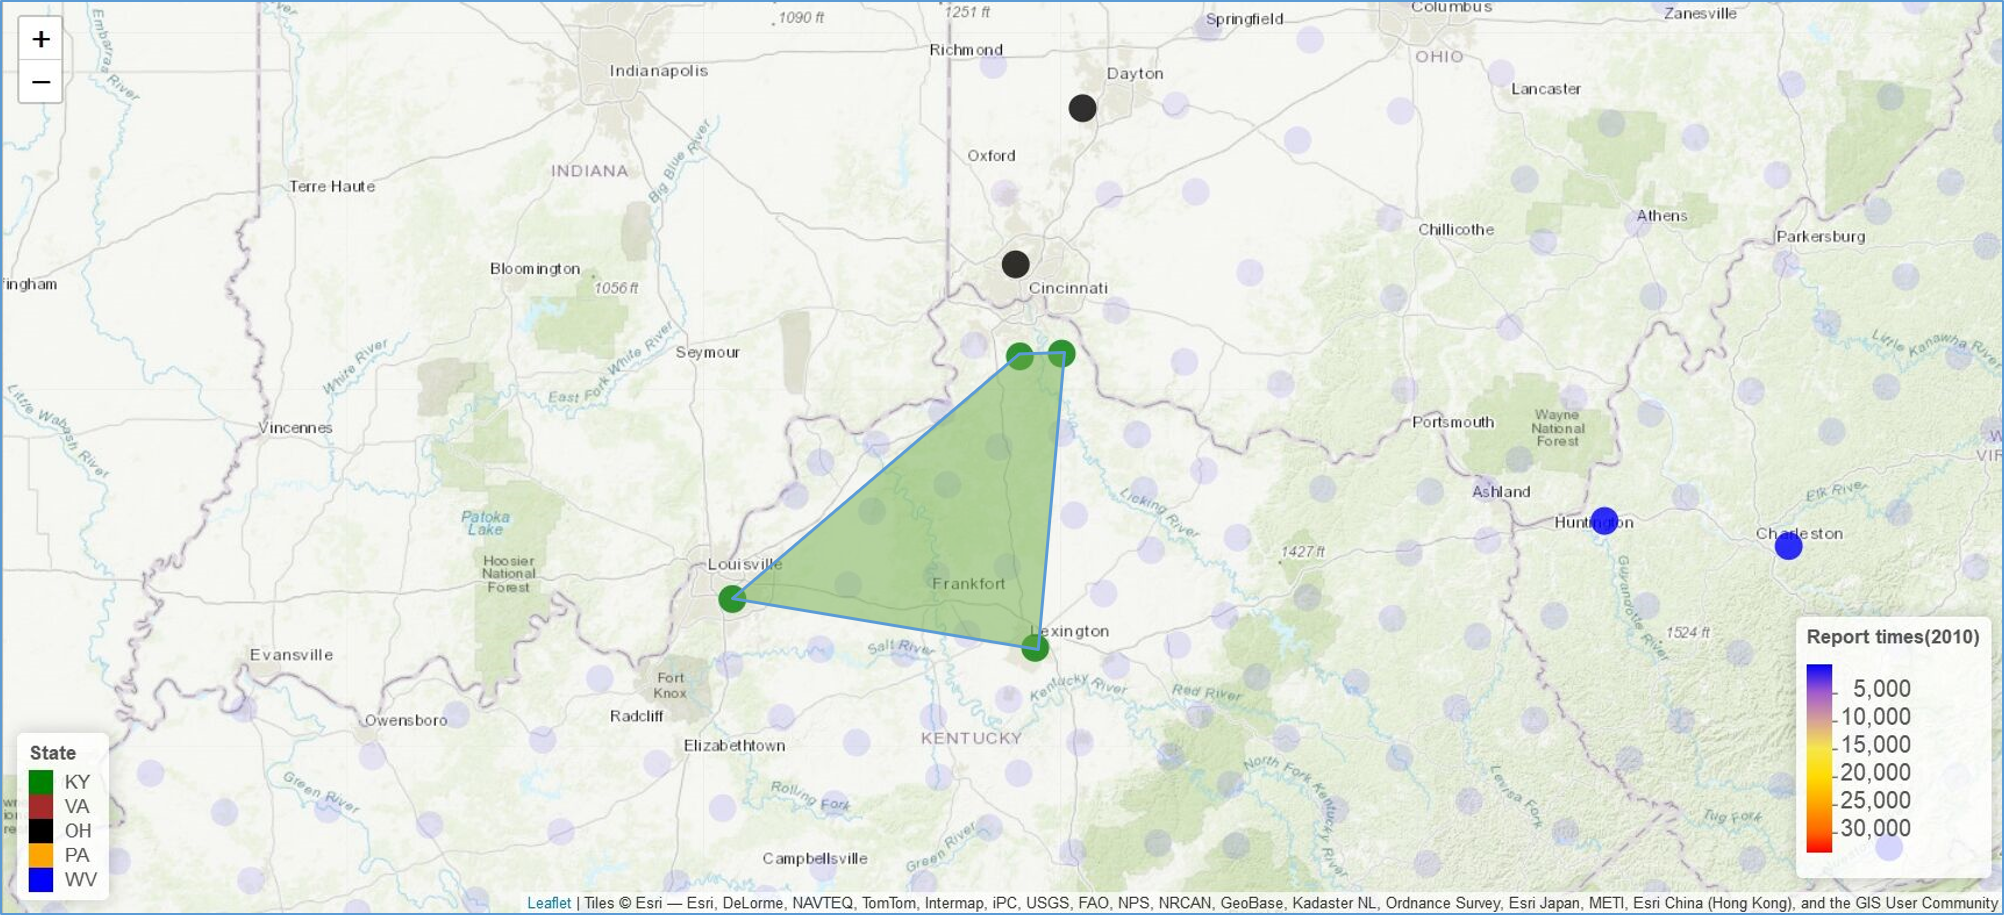
\includegraphics[width=13cm]{Vis}
     	\caption{The Geometric Center of Gravity of the Polygon} \label{fig:Vis}
     \end{figure}
     %%%%% 
\noindent According to The Geometric Center of Gravity Model which is be proposed by us.The four vertices of a polygon are consist of four geographic coordinates to infer to geometric center of gravity.So we can know where the earliest counties to use opioids were reported in five states.\\
    %%根据上述提出的多边形几何重心的模型,四个地理坐标构成多边形的四个顶点,进一步求出多边形的几何重心,就能确定在五个州之内被报道最早使用阿片类药物的县是哪里。
       
     Finally,we need to use the 8 years from 2010 to 2017 as the time variable and the total number of drug reports county as independent variables. Marking 8 geometric centers of gravity on the map.The areas where the earliest use of opioids in these 8 years are covered by these 8 geometric centers of gravity.Otherwise stated, The geometric center of gravity will always be moved on the map.\\
    %%最后,我们将这八个几何重心的坐标在地图上标出,所覆盖的区域表示在这八年内最可能是最早使用阿片类药物的地区。同时,我们观察到,在一定的误差范围内,几何重心总会发生移动
\end{itemize}    
\newpage
%%这是2010和2011的用药情况
\noindent   Here is the ranking of the total drug reports country in 2010 and 2011. \\    
%%%%八张图 2010 和 2011 %%%%%%%%%%%%%%%%%%%%%%%%%%%%%%%%%%%%%
\begin{figure}[htbp]
	\centering
	\subfigure[The top 4 counties of the total drug reports datas in five states in 2010.]{
		\begin{minipage}[t]{0.55\linewidth}
			\centering
			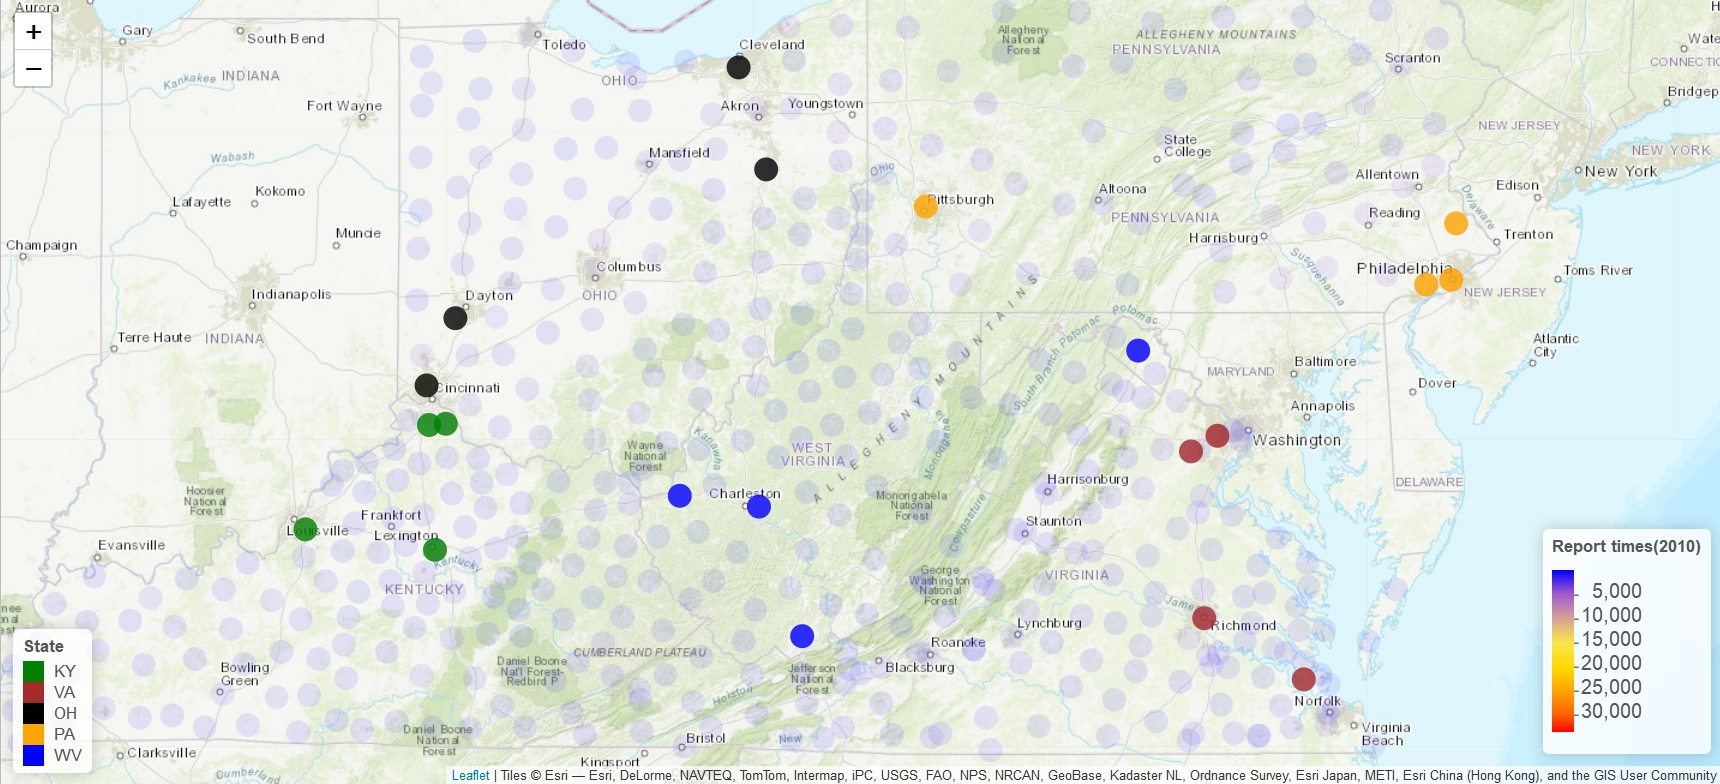
\includegraphics[width=8cm,height=4cm]{2010}
			%\caption{The top 4 counties of the total drug reports datas in five states in 2010}
		\end{minipage}%
	}%
	\subfigure[The top 4 counties of the total drug reports datas in five states in 2011.]{
		\begin{minipage}[t]{0.45\linewidth}
			\centering
			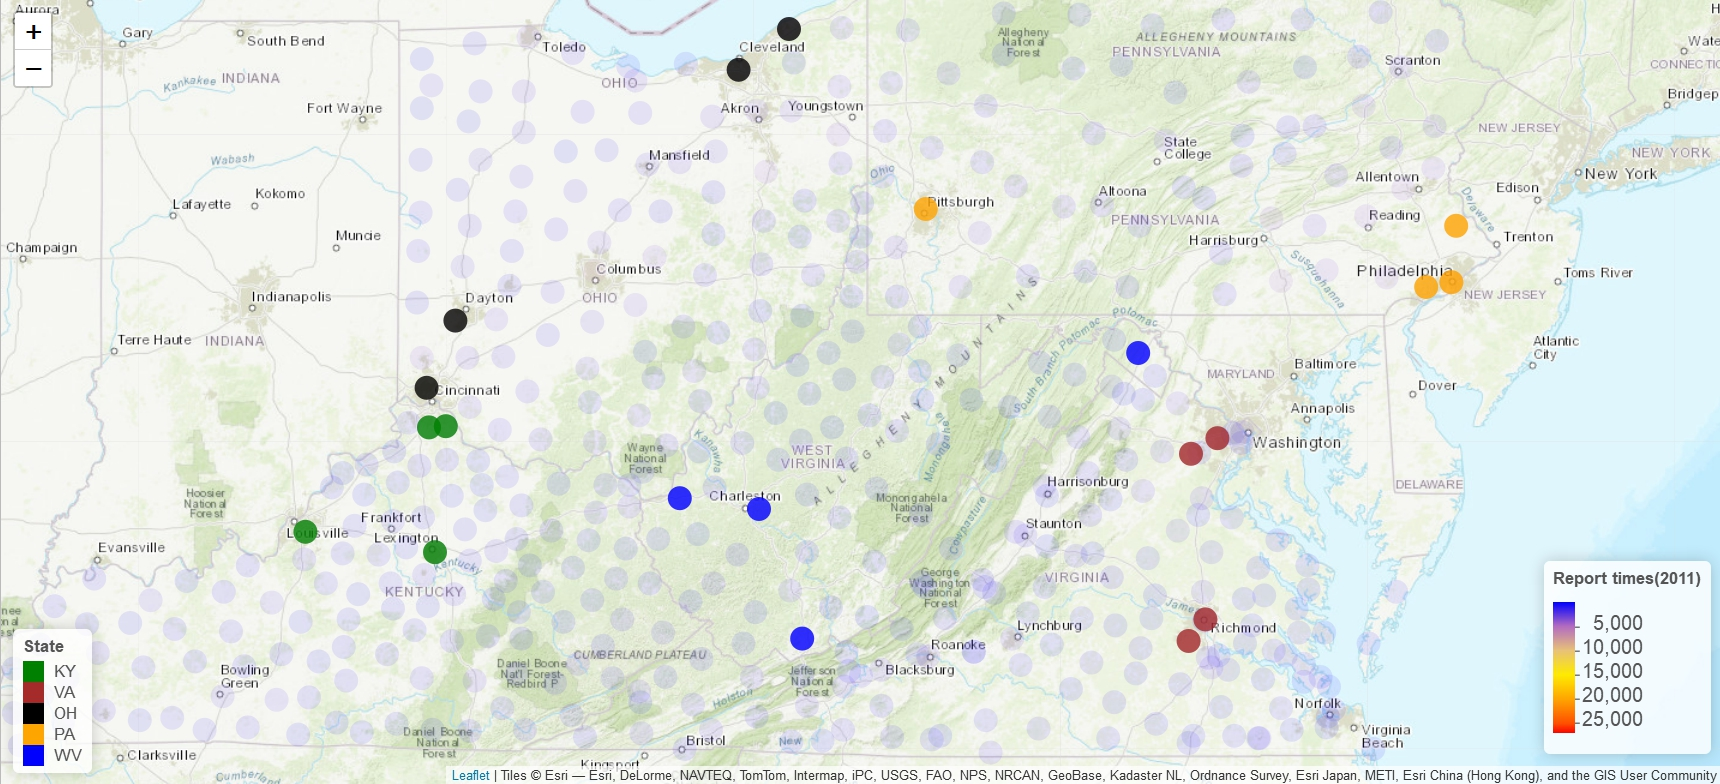
\includegraphics[width=8cm,height=4cm]{2011}
			%\caption{The top 4 counties of the total drug reports datas in five states in 2011}
		\end{minipage}%
	}%
\end{figure}\\
%%这是2012和2013的用药情况
\noindent Here is the ranking of the total drug reports country in 2012 and 2013.\\
%%%%%%%%%%%%%% 2012 和 2013 %%%%%%%%%%%%%%%%%%%
\begin{figure}[htbp]
	\centering
	\subfigure[The top 4 counties of the total drug reports datas in five states in 2012.]{
		\begin{minipage}[t]{0.55\linewidth}
			\centering
			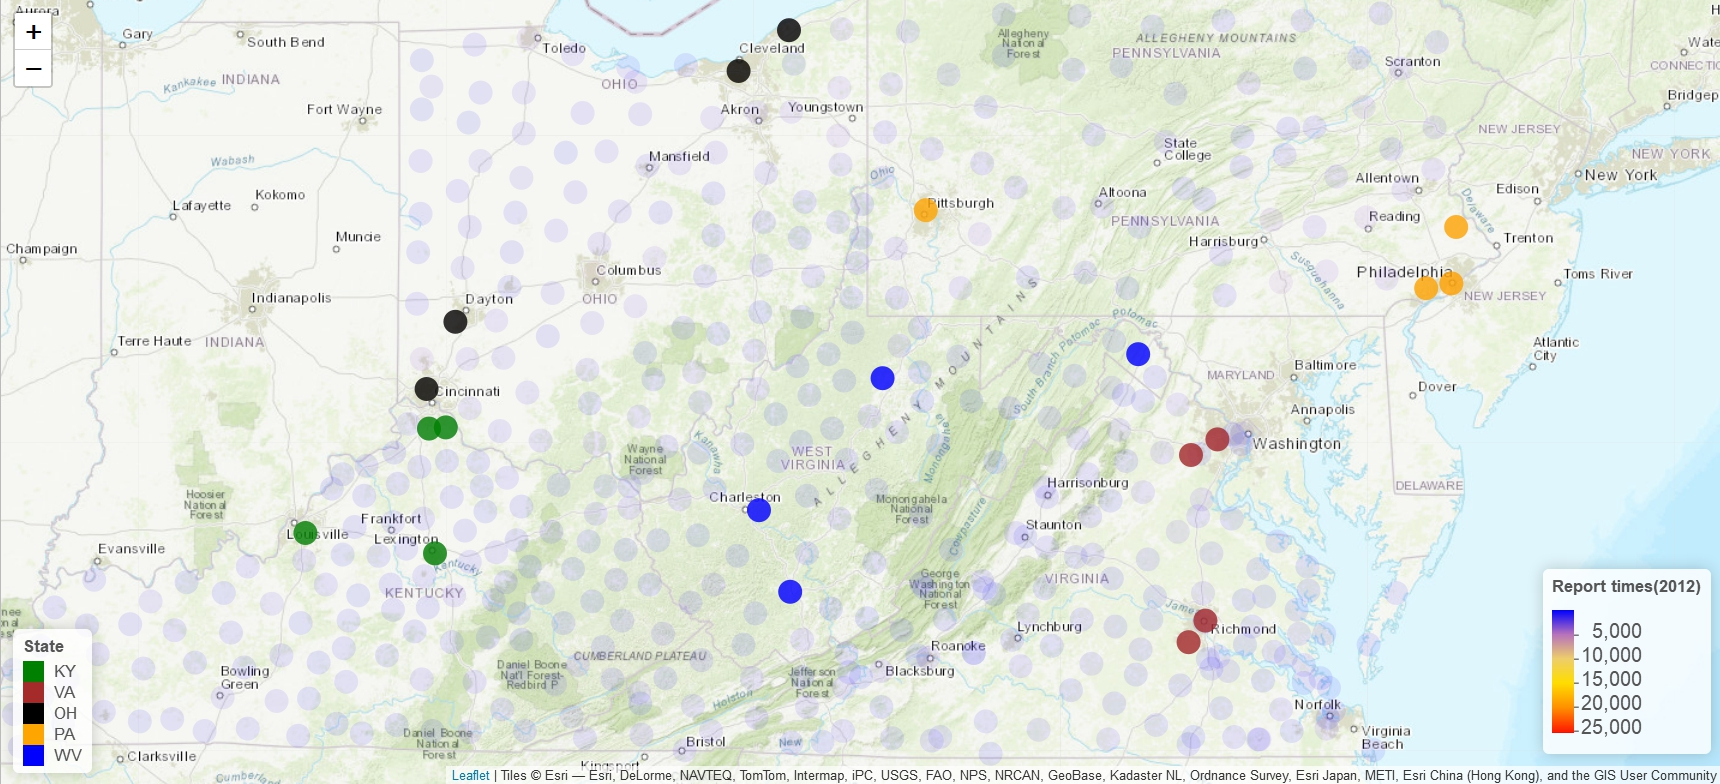
\includegraphics[width=8cm,height=4cm]{2012}
			%\caption{The top 4 counties of the total drug reports datas in five states in 2010}
		\end{minipage}%
	}%
	\subfigure[The top 4 counties of the total drug reports datas in five states in 2013.]{
		\begin{minipage}[t]{0.45\linewidth}
			\centering
			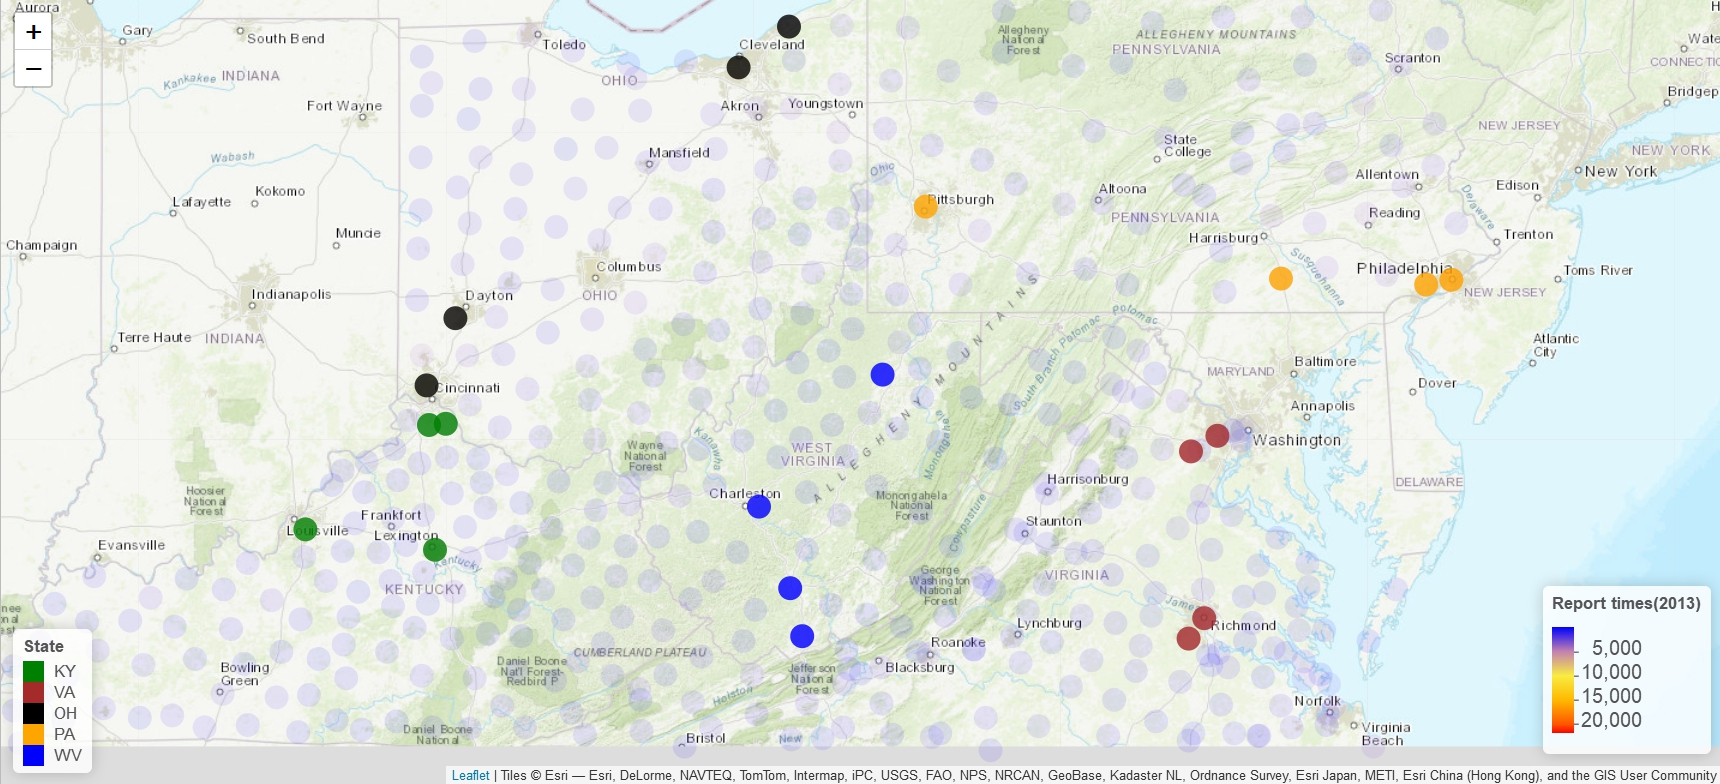
\includegraphics[width=8cm,height=4cm]{2013}
			%\caption{The top 4 counties of the total drug reports datas in five states in 2011}
		\end{minipage}%
	}%
\end{figure}\\
    %%%%八张图%%%%
 %%这是2014和2015的用药情况
 \noindent Here is the ranking of the total drug reports country in 2014 and 2015.\\
 %%%%%%%%%%%%%% 2012 和 2013 %%%%%%%%%%%%%%%%%%%
 \begin{figure}[htbp]
 	\centering
 	\subfigure[The top 4 counties of the total drug reports datas in five states in 2014.]{
 		\begin{minipage}[t]{0.55\linewidth}
 			\centering
 			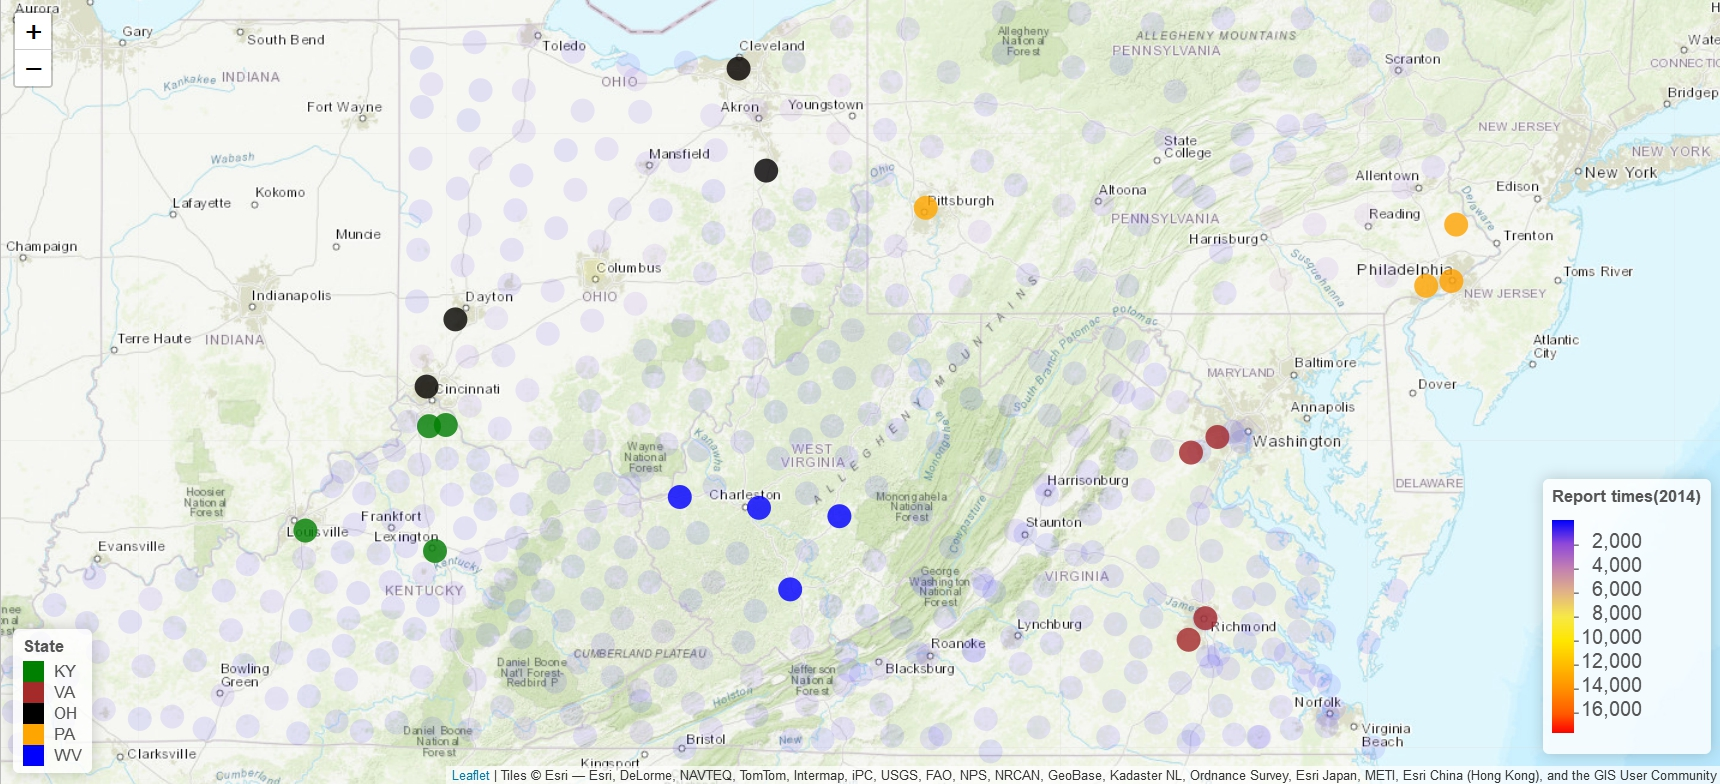
\includegraphics[width=8cm,height=4cm]{2014}
 			%\caption{The top 4 counties of the total drug reports datas in five states in 2010}
 		\end{minipage}%
 	}%
 	\subfigure[The top 4 counties of the total drug reports datas in five states in 2015.]{
 		\begin{minipage}[t]{0.45\linewidth}
 			\centering
 			\includegraphics[width=8cm,height=4cm]{2015}
 			%\caption{The top 4 counties of the total drug reports datas in five states in 2011}
 		\end{minipage}%
 	}%
 \end{figure}\\
\newpage
  %%这是2016和2017的用药情况
 \noindent Here is the ranking of the total drug reports country in 2016 and 2017.\\
 %%%%%%%%%%%%%% 2016 和 2017 %%%%%%%%%%%%%%%%%%%
 \begin{figure}[h]
 	\centering
 	\subfigure[The top 4 counties of the total drug reports datas in five states in 2016.]{
 		\begin{minipage}[t]{0.55\linewidth}
 			\centering
 			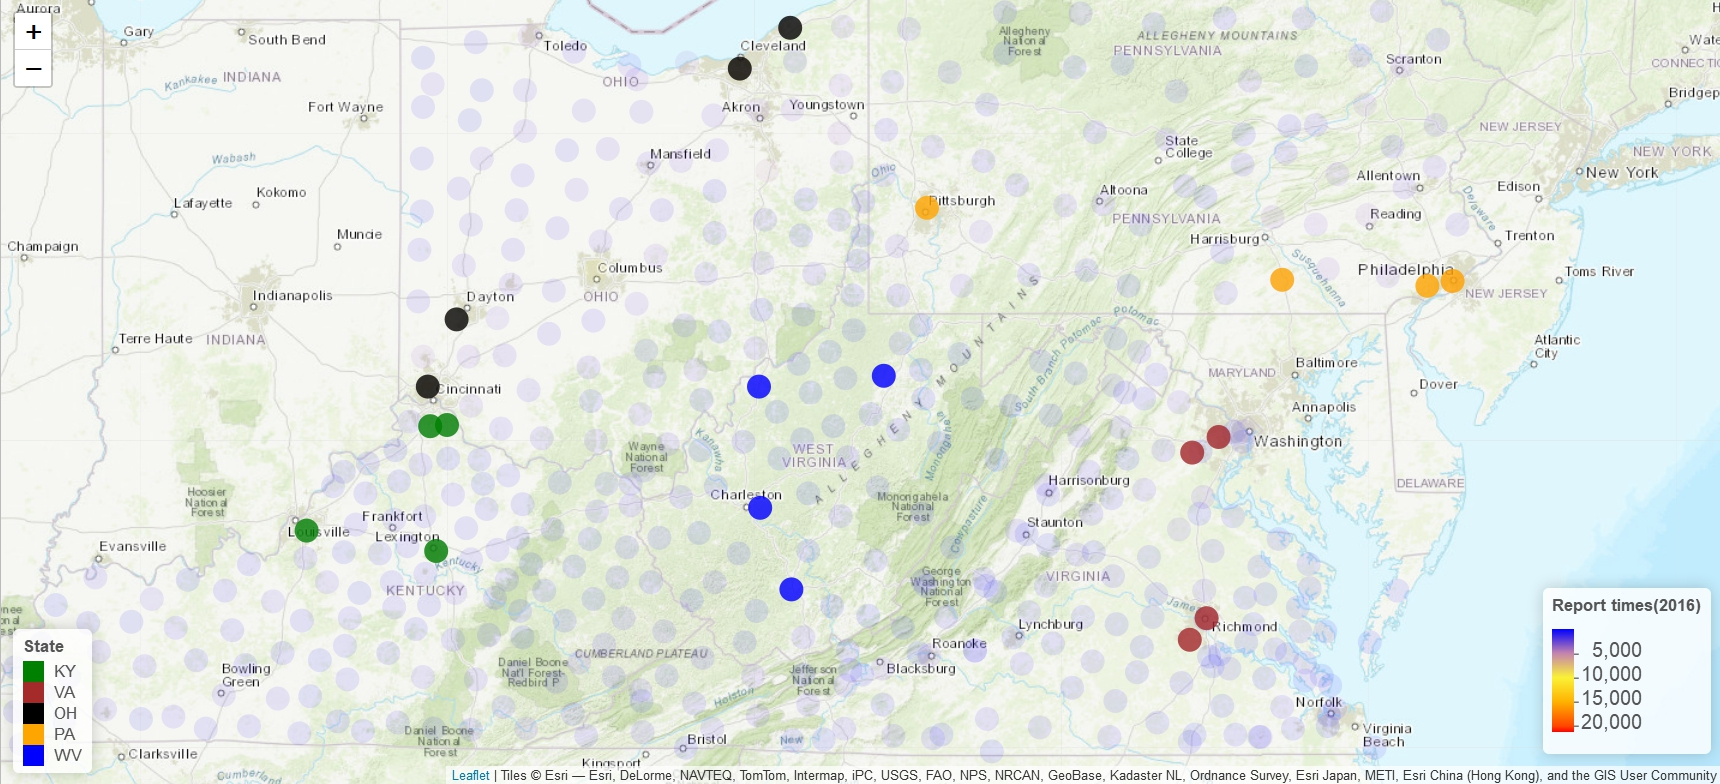
\includegraphics[width=8cm,height=4cm]{2016}
 			%\caption{The top 4 counties of the total drug reports datas in five states in 2010}
 		\end{minipage}%
 	}%
 	\subfigure[The top 4 counties of the total drug reports datas in five states in 2017.]{
 		\begin{minipage}[t]{0.45\linewidth}
 			\centering
 			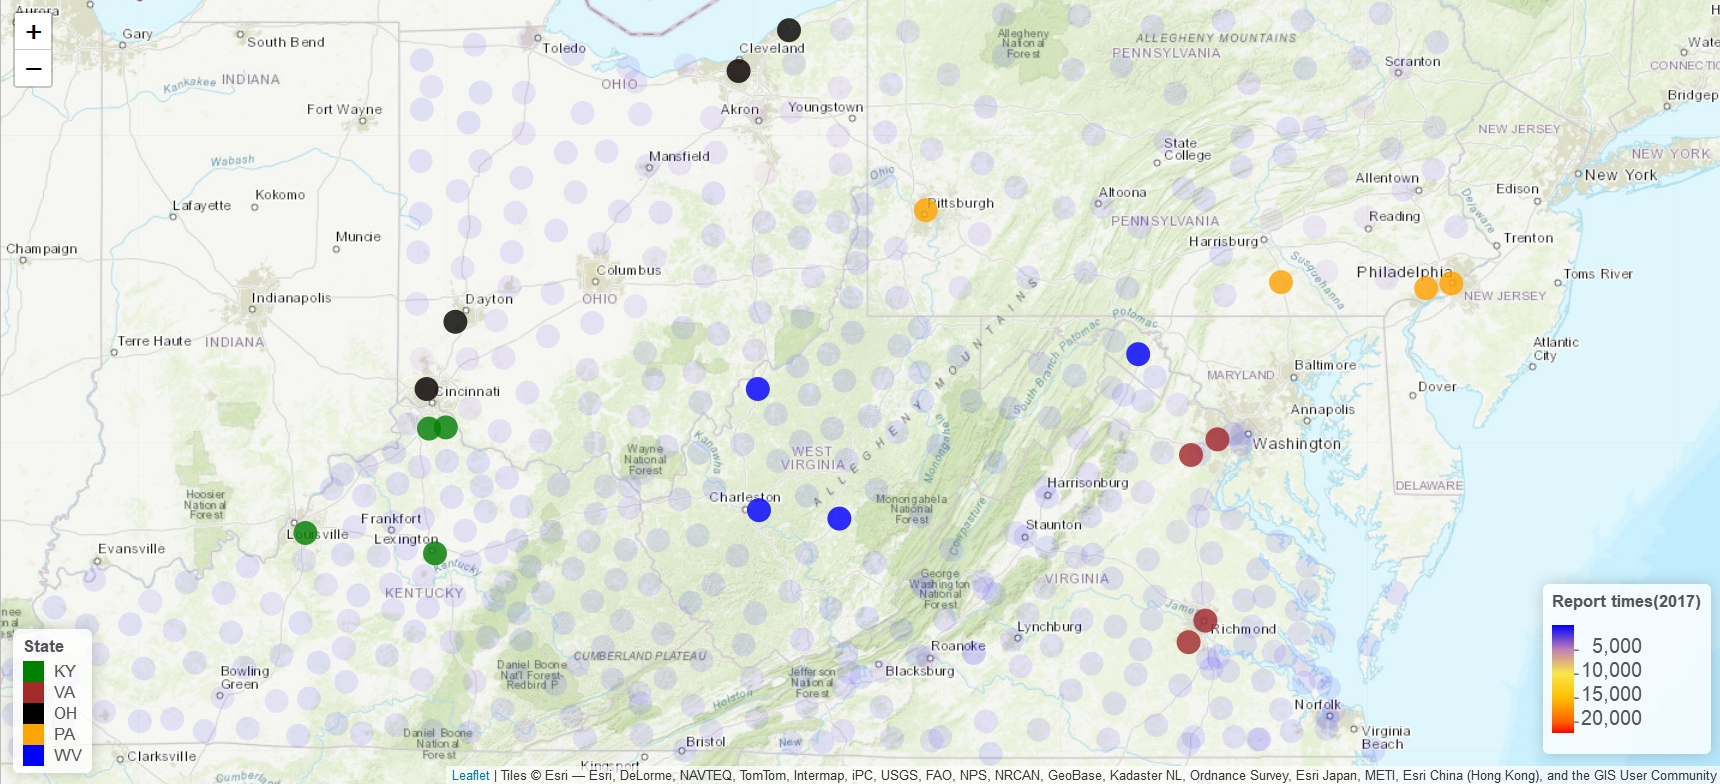
\includegraphics[width=7.5cm,height=4cm]{2017}
 			%\caption{The top 4 counties of the total drug reports datas in five states in 2011}
 		\end{minipage}%
 	}%
 \end{figure}\\   
%%%%%%%插八张图并排显示%%%%%%%%%%%写完再排版%%%%%%%%%
%%%%%%% West Virginia 西弗吉尼亚州(WV) %%% Ohio 俄亥俄州(OH) %%% Kentucky 肯塔基州(KY) %%% Pennsylvania 宾夕法尼亚州(PA)%%% Virginia 吉弗尼亚州(VA) %%%%%
%%%%%%%%%%%%%%%%%%%%%%%%%%%%%%%%%%%%%%%%%%%%%%%%%%%%%%%%%%%%%%%%%%%%%%%%%%%%
%%根据多边形几何重心模型,我们可以直观地看出每一年分布在 WV、OH、KY、PA、VA这五个州用药总数排名靠前的四个县城分别是(每一年份)。五个州
%%%%%经纬度这里就是模型一的答案%%%%%%
% Table generated by Excel2LaTeX from sheet 'Sheet1'
\begin{table}[htbp]
	\centering
	\caption{The location of the state that was the earliest reported to use opioids}
	\begin{tabular}{p{5cm}p{5cm}p{3cm}} %%设置宽度
		\addlinespace
		\toprule
		State & Longitude   & Latitude \\
		\midrule
		KY    & \ang{84.89390718}W & \ang{38.34210878}N\\ 
		VA    & \ang{77.54358872}W & \ang{38.26026487}N\\
		WV    & \ang{80.12507797}W & \ang{38.59615550}N \\
		OH    & \ang{83.22998974}W & \ang{40.21617205}N\\
		PA    & \ang{77.01509742}W & \ang{40.18737616}N \\
		\bottomrule
	\end{tabular}%
	\label{tab:addlabel}%
\end{table}%

%%%%%%%%%%%%%%%%%%%%%%%%%%%
\noindent According to the polygonal geometric center of gravity model,we can observe clearly the top 4 counties associate with 4 vertexs of the total drug reports datas in five states every year.And the five states have five geometric centers of gravity on map.So there are some longitude and latitude coordinates in five states.\\
%%%%%%%
%%最后,我们将这八年的用药总数进行求和
\noindent At the end,we add and average the eight years of the total drugs reports data to get longitude and latitude coordinates.\\

\noindent Here are the latitude and longitude of the four geometric centers.The geometric centers stand for \textbf{the location which the earliest use of opioids}.\\

\subsection{Model 2 - The Grey Models for Short-term Predicts Solution}%%模型二 灰色模型的求解 
\noindent According to the gray model,we intend to sum up the total drug data for eight years.Here is the total drug data table for \textbf{eight years}.\\%%%根据模型二,我们只将每个县和它有关联的州进行联系,将所有年用药数据总和相加,就可以得到该州的第 n 年的阿片类药物总和。
%%%总和的三线表 %%%%%%
\begin{center}
	\textbf{Table 1}~~The total drug data about all years.\\%%五个州的八年用药总和 编号自定义需要重新改
	\resizebox{\textwidth}{15mm}{
	%\caption{the total drug data about all years.}%%
\begin{tabular}{|c|c|c|c|c|c|c|c|c|} 
	\hline 
	 \diagbox{State}{Year} &2010&2011&2012&2013&2014&2015&2016&2017 \\ 
	  \hline 
	  KY    &10453&10289&10722&11148& 11081 & 9865  & 9093  & 9394 \\
	  OH    &19707&20330&23145&26846& 30860 & 37127 & 42470 & 46104 \\
	  PA    &19814&19987&19959&20409& 24904 & 25651 & 26164 & 27894 \\
	  VA    &8685&6749&7831&11675&9037  & 8810  & 10195 & 10448 \\
	  WV    &2890&3271&3376&4046&3280  & 2571  & 2548  & 1614 \\	  
	    \hline 
     \end{tabular}}
\end{center}
%%%% 总和的三线表 %%%%%%
\noindent We use the gray model to predict the tatal drugs data about all years.As long as we have already gotten the Grey-correlation of each data.\\%%我们使用灰色模型对上述数据分别预测得到每个州的灰色关联度数据
%%%%%%%%%%灰色关联度%%%%%%%%%%%
\begin{table}[htbp]
	\centering
    \caption{Gray-correlation of each state} %% 预测2018年之后的三年 
	\begin{tabular}{p{4cm}p{4cm}p{4cm}}\toprule 
		State & Grey-correlation & Precision $ \le 0.35$\\ \midrule 
		PA & excellent & 0.178 \\
		OH & excellent & 0.059\\ 
		WV & average & 0.457\\
		KY & fair & 0.518\\
		VA & poor & 0.665\\
		\bottomrule
	\end{tabular} 
\end{table}
%%%%%%%%%%%%%灰色关联度%%%%%%%%%%%%%%%

\noindent In this table.If the gray correlation is more lower,Then the predictive value will get more acurrate.We can draw some important conclusions.\\
%%%%% 结论分点 %%%%%%%
\begin{itemize}
	\item The total drug reports is more higher in the Pennsylvania and Ohio\\%PA和OH的预测值精确度较高
	\item The total drug reports is more lower in the Kentucky\\%KY的预测值精确度较低
	\item The total drug reports is general in the West Virginia.\\%WV的预测值精确度中等
	\item The total drug reports is the lowest in the Virginia.\\%VA的预测值精确度最低
\end{itemize}
%%%%%%%%这里是关于五个州的数据表 %%%%%%%%%%%
There are some charts about the ratio between predictive value and original value.\\
%%%%%% 五个州的灰色预测 %%%%%% 
%%%%%%%%%%% PA %%%%%%%%%% 可以和 Logistic 结论吹 %%%%%
\begin{figure}[!h]
	\centering
	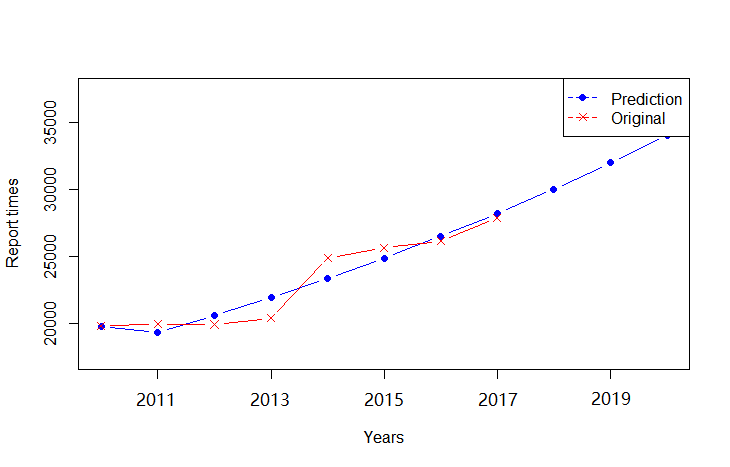
\includegraphics[height=6cm,width=14cm]{pa}
	\caption{PA}
	\label{PA}
\end{figure}
%%%%%% OH and WV %%%%%%%
 \begin{figure}[htbp]
	\centering
	\subfigure[OH]{
		\begin{minipage}[t]{0.55\linewidth}
			\centering
			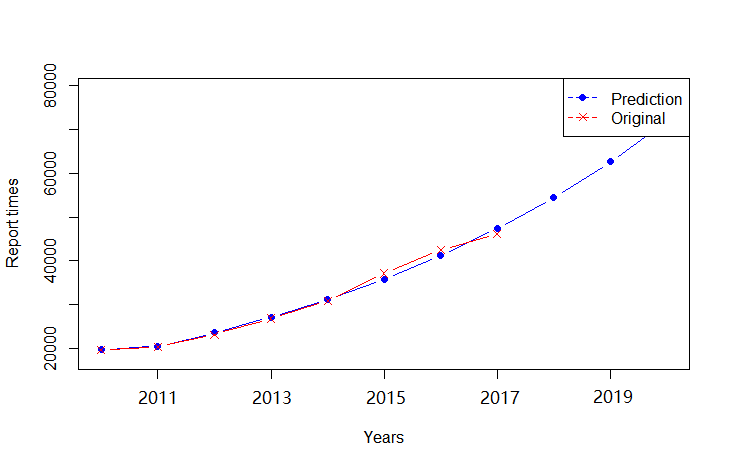
\includegraphics[width=8cm,height=4cm]{oh}
			%\caption{The top 4 counties of the total drug reports datas in five states in 2010}
		\end{minipage}%
	}%
	\subfigure[VA]{
		\begin{minipage}[t]{0.55\linewidth}
			\centering
			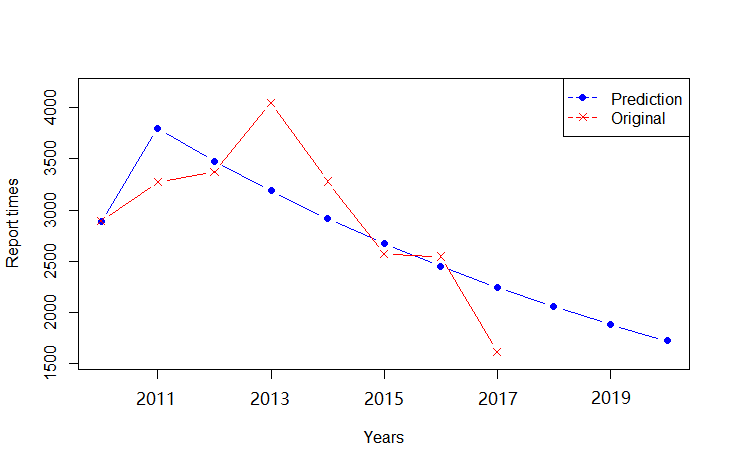
\includegraphics[width=8cm,height=4cm]{wv}
			%\caption{The top 4 counties of the total drug reports datas in five states in 2011}
		\end{minipage}%
	}%
\end{figure}
%%%%%% KY and VA %%%%%%%
 \begin{figure}[htbp]
	\centering
	\subfigure[KY]{
		\begin{minipage}[t]{0.55\linewidth}
			\centering
			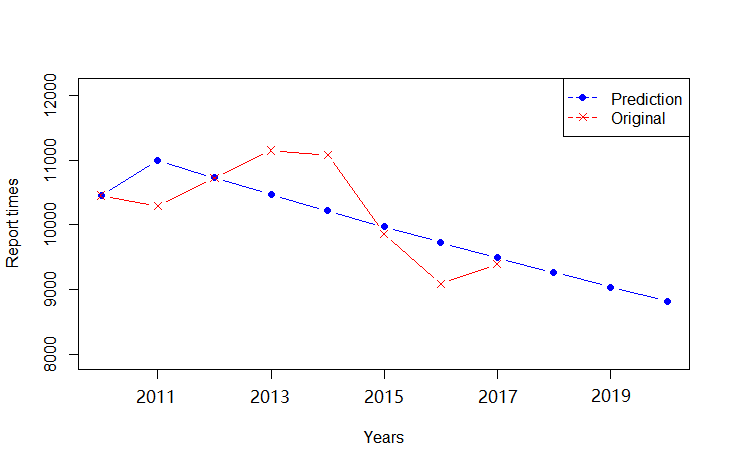
\includegraphics[width=8cm,height=4cm]{ky}
			%\caption{The top 4 counties of the total drug reports datas in five states in 2010}
		\end{minipage}%
	}%
	\subfigure[WV]{
		\begin{minipage}[t]{0.55\linewidth}
			\centering
			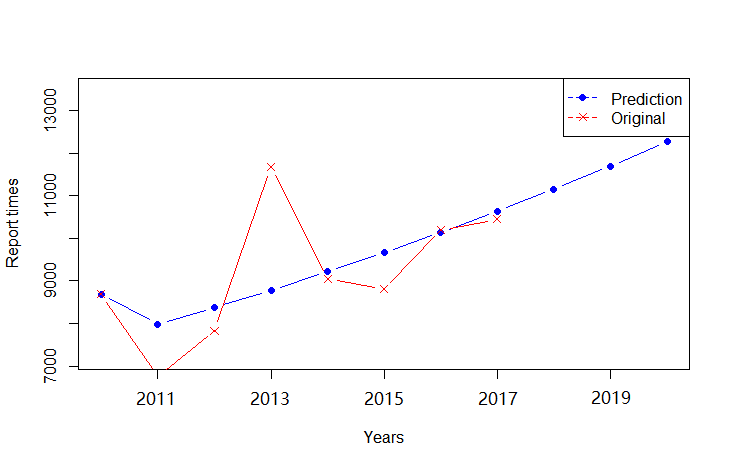
\includegraphics[width=8cm,height=4cm]{va}
			%\caption{The top 4 counties of the total drug reports datas in five states in 2011}
		\end{minipage}%
	}%
\end{figure}
%%%%%% 五个州的灰色预测 %%%%%%%
\newpage
\subsection{Model 3 - The Logistic Regression for Medium-term  Predicts Solution} %%模型三求解 Logistic回归模型中期预测
\noindent According to the sample data is single,We found that the prediction using the GM model is not very good.So we dicided to use the Logistic Regression predicted the total drug reports situation.%%根据模型三的求解结果,我们得出使用灰色预测模型进行短期预测用药总数的结果效果很好,由于样本数据的单一,灰色预测在中期和长期预测中预测效果不好。于是我们选择使用 Logistic 回归模型进行中期预测,优化现有的模型。
\begin{figure}[!h] %浮动位置
	\small
	\centering
	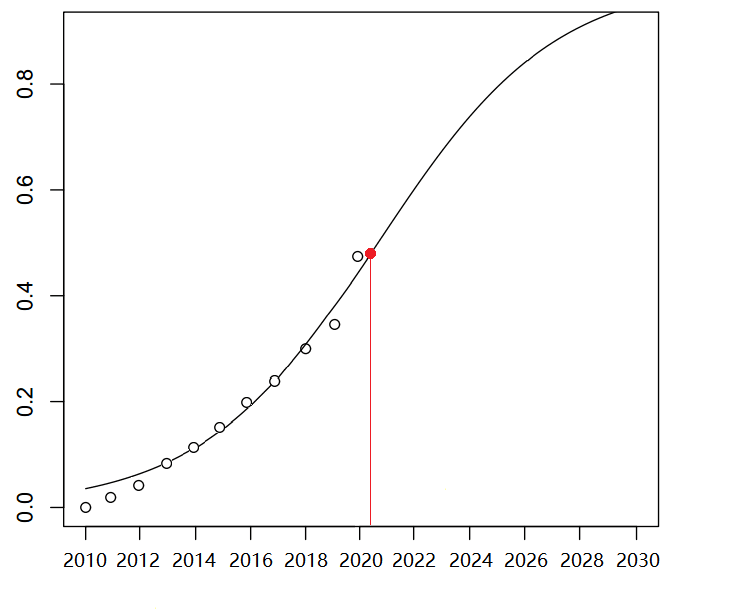
\includegraphics[width=10cm,height=8cm]{logict}
	\caption{The logistic regression predicted total drug reports situation in 2010 to 2020. } %%
	 \label{fig:Vis}
\end{figure}
In this table,we can draw some important conclusion.
%%在这张图中,我们可以得出一些重要的结论
\begin{itemize}
	\item The small dots is raw data before 2017.And the small dots is predictive data in 2017 to 2020.%%2017年之前是原始数据,2017年之后是预测数据
	\item If the X-axis is 2020,Then the Y-axis means that is the highest drug identification threshold levels. %%在2020年处是拐点,发生变化,我们必须提醒美国政府这可能是药物识别阈值水平,需要在2020和2021年之间警惕阿片类药物的滥用情况。
	\item This table approximate to gray model prediction results in the Pennsylvania.  %%与灰色模型预测作比较,logistc回归模型预测的结果近似于灰色模型预测的结果。。(对于PA州而言,呈指数增长)
\end{itemize}

\subsection{Model 4 - The BP Artificial Neural Network predicts the next new disaster location} %%模型四求解 The BP Artificial Neural Network predicts the next new disaster location .KY!!!
%%%%%%%%%%%%%% BP 的求解 %%%%%%%%%%%
\begin{itemize}
	 \item  For each states, $h$ means input variable.
\begin{itemize}
	\item[-] $h_1$ means the coordinates of the top 20 counties in 2010 to 2014.\\%2010-2014
	\item[-] $h_2$ means the coordinates of the top 20 counties in 2011 to 2015. \\
	\item[-] $h_3$ means the coordinates of the top 20 counties in 2012 to 2016. \\
\end{itemize}
\end{itemize}
%%根据模型四,我们能够使用 BP 人工神经网络 预测下一个滥用阿片类药物的爆发地点。对于每个州,h作为输入变量,h1取2010~2014年排名靠前20的县的坐标点信息;h2取2011-2015年排名靠前20县的信息,h3取2012~2016年排名靠前的20的县坐标信息。target作为自变量y,y取2013~2017年排名前20的县的坐标。这样就构成了一个自我学习的神经网络。我们将各项数据放入 MATLAB 进行训练,得到误差(纵坐标)和迭代次数(横坐标)的图像。
\begin{itemize}
	\item  If $ epochs$ = 16, the next most likely location for an opioid crisis will appear.%% 由预测曲线可知,发生变化将会在迭代次数 16 时发生变化,确定下一个位置的产生趋势	
	\item From the data in the table, we can see that the next geographical location where drug abuse occurs is Kentucky.%% 由坐标数据可知,预测下一个分布位置是 KY
\end{itemize}
%%图像
\begin{figure}[!h] %浮动位置
	\small
	\centering
	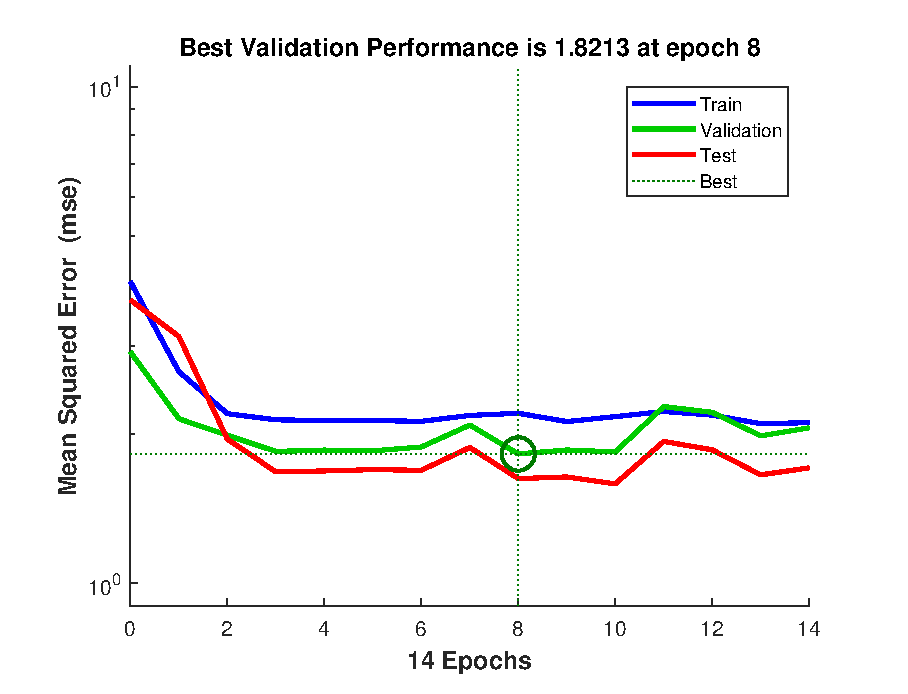
\includegraphics[width=10cm,height=8cm]{BP}
	\caption{The BP artificial neural network predicts the geographical position of 20 counties.} %%
	\label{fig:BP}
\end{figure}

%%预测的经纬度坐标(可以插在附录)20组
%%% sheet 1
% Table generated by Excel2LaTeX from sheet '1'
\begin{table}[htbp]
	\centering
	\caption{Predicting the next geographic location where abuse of opioids occurs.}
	\begin{tabular}{rrrrrr}
		\addlinespace
		\toprule
		longitude & \ang{85.604}W & \ang{84.386}W & \ang{84.535}W & \ang{84.424}W & \ang{83.557}W \\
		\midrule
		latitude & \ang{38.085}N & \ang{38.074}N & \ang{38.941}N & \ang{38.926}N & \ang{36.746}N \\
		\bottomrule
	\end{tabular}%
	\label{tab:addlabel}%
\end{table}%
%%% sheet 2
% Table generated by Excel2LaTeX from sheet '1'
\begin{table}[htbp]
	\centering
	\caption{Predicting the next geographic location where abuse of opioids occurs.}
	\begin{tabular}{rrrrrr}
		\addlinespace
		\toprule
		longitude & \ang{85.959}W & \ang{84.3}W & \ang{87.046}W & \ang{84.141}W & \ang{86.516}W \\
		\midrule
		latitude & \ang{37.611}N & \ang{37.755}N & \ang{37.667}N & \ang{37.198}N & \ang{37.058}N \\
		\bottomrule
	\end{tabular}%
	\label{tab:addlabel}%
\end{table}%
%%% sheet 3
% Table generated by Excel2LaTeX from sheet '1'
\begin{table}[htbp]
	\centering
	\caption{Predicting the next geographic location where abuse of opioids occurs.}
	\begin{tabular}{rrrrrr}
		\addlinespace
		\toprule
		longitude & \ang{84.633}W & \ang{88.791}W & \ang{85.507}W & \ang{84.667}W & \ang{83.243}W \\
		\midrule
		latitude & \ang{39.018}N & \ang{36.986}N & \ang{37.844}N & \ang{37.157}N & \ang{37.251}N \\
		\bottomrule
	\end{tabular}%
	\label{tab:addlabel}%
\end{table}%
%%% sheet 4
% Table generated by Excel2LaTeX from sheet '1'
\begin{table}[htbp]
	\centering
	\caption{Predicting the next geographic location where abuse of opioids occurs.}
	\begin{tabular}{rrrrrr}
		\addlinespace
		\toprule
		longitude & \ang{82.696}W & \ang{87.518}W & \ang{83.149}W & \ang{82.725}W & \ang{85.768}W \\
		\midrule
		latitude & \ang{38.417}N & \ang{37.381}N & \ang{36.808}N & \ang{37.487}N & \ang{38.024}N \\
		\bottomrule
	\end{tabular}%
	\label{tab:addlabel}%
\end{table}%

%%结论
\newpage
\subsection{Model 5 - The Factor Analysis process the multidimensional data}%% 使用因子分析处理多维数据
%%%%%%%%%%%%% 因子分析 %%%%%%%%%%%%%%%%%%%%%%%%

For question two, we need to use the socio-economic data from the US Census to analyze the combined causes of the crisis of opioid abuse.Our team observed that this is a very large amount of data, so we will use a factor analysis method to reduce it.
%%对于问题二,要求我们需要利用美国人口普查的社会经济数据去分析造成阿片类药物滥用危机的综合原因。我们小组观察到这个是一个十分庞大的数据,所以采用因子分析的办法对其进行降维处理。

Take the socioeconomic data of the 2010 American Census as an example,we cleaned this data.When choosing the number of load factors, we find that it is feasible to use two factors to indicate the degree of correlation between data.
%%以2010年的美国人口普查的社会经济数据为例,随后进行数据清洗。在我们选择载荷因子个数时,发现用两个因子表示因素之间的代表程度更适合,贡献度高达 80%

% Table generated by Excel2LaTeX from sheet 'Sheet1'
\begin{table}[htbp]
	\centering
	\caption{Five load factors contribution}
	\begin{tabular}{rrrrrr}
		\addlinespace
		\toprule
		& Factor1 & Factor2 & Factor3 & Factor4 & Factor5 \\
		\midrule
		SS loadings  & 137.677 & 73.618 & 10.505 & 6.19  & 10.784 \\
		Proportion Var  & 0.499 & 0.267 & 0.038 & 0.022 & 0.039 \\
		Cumulative Var  & 0.499 & 0.766 & 0.804 & 0.826 & 0.865 \\
		\bottomrule
	\end{tabular}%
	\label{tab:factor}%
\end{table}%

We can draw an important conclusion that Factor 1 and Factor 2 can respectively distinguish the US population data into two dimensions.At the same time, their cumulative contribution reached 80 percent.Factor 1 represents a group of people with poor marital status and parenting.but Factor 2 represents unmarried and children without children. 
%%% 从表中可以看出 载荷因子1和载荷因子2 的累加贡献度(Cumxxxx)高达 80%,我们可以得出一个结论。两个载荷因子能够分别

%%绘制人口数据在这两个载荷因子的分布图
\begin{figure}[!h] %浮动位置
	\small
	\centering
	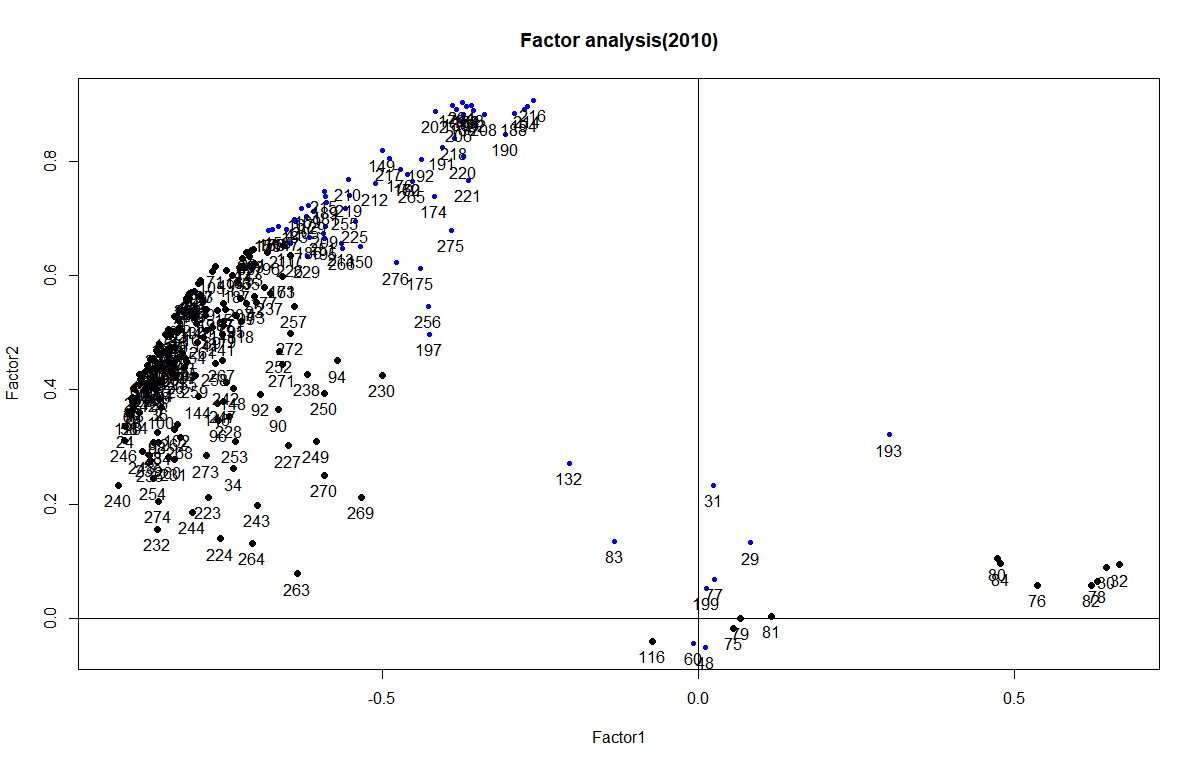
\includegraphics[width=10cm,height=8cm]{Factor}
	\caption{Distribution of population data in two load factors} %%
	\label{fig:Factor}
\end{figure}
%%%%%%%%%%%%%











%%%%%%%%%%%%%%%%%%%%%%%%%%%%%%%%%%%%%%%%%%%%%%%%
\section{Strengths and weaknesses} %%模型优点和缺点





%%%%%%插入文献%%%%%%
\begin{thebibliography}{99}
\bibitem{1} D.~E. KNUTH   The \TeX{}book  the American
Mathematical Society and Addison-Wesley
Publishing Company , 1984-1986.
\bibitem{2}Lamport, Leslie,  \LaTeX{}: `` A Document Preparation System '',
Addison-Wesley Publishing Company, 1986. 
\bibitem{3}\url{http://www.latexstudio.net/}
\bibitem{4}\url{http://www.chinatex.org/}
\end{thebibliography}


%%%%%%附录代码%%%%%%
\begin{appendices}

\section{First appendix}

Here are simulation programmes we used in our model as follow.\\

\textbf{\textcolor[rgb]{0.98,0.00,0.00}{Input matlab source:}}
\lstinputlisting[language=Matlab]{./code/mcmthesis-matlab1.m}


\section{Second appendix}
some more text \textcolor[rgb]{0.98,0.00,0.00}{\textbf{Input C++ source:}}
\lstinputlisting[language=C++]{./code/mcmthesis-sudoku.cpp}
\end{appendices}
\end{document}



%%
%% This work consists of these files mcmthesis.dtx,
%%                                   figures/ and
%%                                   code/,
%% and the derived files             mcmthesis.cls,
%%                                   mcmthesis-demo.tex,
%%                                   README,
%%                                   LICENSE,
%%                                   mcmthesis.pdf and
%%                                   mcmthesis-demo.pdf.
%%
%% End of file `mcmthesis-demo.tex'.
